% Thanks to Samuel Charreyron and his Data Mining cheat sheet for the layout! :)

\documentclass[7pt,parskip]{scrartcl}
\usepackage{calc}
\usepackage[landscape,paper=a4paper,left=3mm, right=3mm,top=0mm, bottom = 3mm,includehead,headheight=5mm,headsep=2mm]{geometry}
\usepackage{multicol}
\usepackage[alwaysadjust]{paralist}
% \usepackage[tight]{savetrees}
\usepackage[ngerman]{babel}
\usepackage[utf8]{inputenc}
\usepackage[T1]{fontenc}
\usepackage{multirow}

\renewcommand\familydefault{\rmdefault}
\usepackage[]{amsmath}
\usepackage{amssymb}
\usepackage{amsfonts}
\usepackage{empheq}
\usepackage{color}
\usepackage{graphicx}
\usepackage{wrapfig}
\usepackage{mdframed}
\usepackage{algorithm}
\usepackage[noend]{algpseudocode}
\usepackage{physics}
\usepackage{hyperref}
\usepackage[dvipsnames]{xcolor} 

\graphicspath{/}

 %PLATZSPAAREN SPACING 
\setlength{\parskip}{0pt}
\setlength{\parsep}{0pt}

\usepackage{mathrsfs}

\usepackage[]{titlesec} % SPACING überall definieren
\titlespacing*{\section}{0pt}{0pt}{5pt} %indent,space befor, space after
\titlespacing*{\subsection}{0pt}{0.2cm}{0pt}
\titlespacing*{\subsubsection}{0pt}{0.15cm}{0pt}
\titleformat*{\section}{\fontencoding{OT1}\fontfamily{cmr} \fontseries{bx}\fontshape{sc} \fontsize{15pt}{15pt} \selectfont\color{Maroon}} %italic
\titleformat*{\subsection}{\fontencoding{OT1}\fontfamily{cmr} \fontseries{bx}\fontshape{sc} \fontsize{10pt}{10pt} \selectfont\color{OliveGreen}} %italic
\titleformat*{\subsubsection}{\fontencoding{OT1}\fontfamily{cmr} \fontseries{bx}\fontshape{sc} \fontsize{9pt}{9pt} \selectfont\color{NavyBlue}} %italic
\def\thesection{}
\def\thesubsection{\arabic{subsection}}

\definecolor{myblue}{cmyk}{1,.72,0,.38}
\everymath\expandafter{\the\everymath \color{myblue}}
\everydisplay\expandafter{\the\everydisplay \color{myblue}}


%% MACROS %%

\def\(({\left(}
\def \xyz{ \(( \begin{array}{ccc }
    x \\
  y \\
  z
\end{array}\))
}
\def \sphere{ \(( \begin{array}{ ccc}
    r \\
  \theta \\
  \phi
\end{array} \))
}
\def\)){\right)}
\newcommand{\diffn}[2]{\frac{d \ #1}{d  #2}}
\newcommand{\diffp}[2]{\frac{\partial  #1}{\partial   #2}}

\newcommand{\myv}[3]{ \(( \begin{array}{ccc}
    #1 \\
  #2 \\
  #3
\end{array}\))
}

\newcommand{\bild}[3]{
\begin{figure}[H]  
 \centering
    \includegraphics[#3]{#1}
    \caption{#2}
\end{figure}
}

\newcommand{\bildlabel}[4]{
\begin{figure}[h]  
 \centering
    \includegraphics[#3]{#1}
    \caption{#2}
    \label{#4}
\end{figure}
}

\newcommand{\bildo}[2]{
\begin{figure}[H]  
 \centering
    \includegraphics[#2]{#1}
\end{figure}
}

\newcommand{\un}{\underline}
%Fr fbox:
\newcommand{\f}{\fbox}


\newcommand{\ra}{\rightarrow}
\newcommand{\s}{\sigma}
\newcommand{\e}{\epsilon}

\newcommand{\al}[1]
{\begin{align*}
#1
\end{align*}
}

\newcommand{\aln}[1]
{\begin{align}
#1
\end{align}
}

%% Emphasize Math ==============================
\definecolor{insidecolor}{rgb}{0.93,0.93,0} 
\definecolor{border}{rgb}{0,0,0}
 
\newcommand*\mybluebox[1]{% 
\fcolorbox{border}{insidecolor}{\hspace{1em}#1\hspace{1em}}
}

\newcommand{\eal}[1]
{\begin{empheq}[box=\mybluebox]{align*} 
#1
\end{empheq}
}

\newcommand{\ealn}[1]
{\begin{empheq}[box=\mybluebox]{align} 
#1
\end{empheq}
}

\newcommand{\emult}[1]
{\begin{empheq}[box=\mybluebox]{multline*} 
#1
\end{empheq}
}
\newcommand{\emultn}[1]
{\begin{empheq}[box=\mybluebox]{multline} 
#1
\end{empheq}
}
%==========================================

\newcommand{\tsf}[1]
{\textsf{#1}
}

\newcommand{\tbf}[1]
{\textbf{#1}
}


\newcommand{\fal}[1]
{\begin{flalign*}
#1
\end{flalign*}
}

\newcommand{\ocirc}[1]{\buildrel _{\circ} \over {\mathbf{#1}}}

\newenvironment{fminipage}%
{\begin{Sbox}\begin{minipage}}%
{\end{minipage}\end{Sbox}\fbox{\TheSbox}}



\newenvironment{mybulletlist}
{%begin
\begin{list}{\RIGHTarrow}
{\setlength{\topsep}{0cm} 
\setlength{\parsep}{2mm}
\setlength{\leftmargin}{1.5cm}
\setlength{\rightmargin}{0cm}
\setlength{\labelwidth}{2cm} 
\setlength{\labelsep}{0.5cm}}
}
{%end
\end{list} 
}

\newcounter{linie}
\newenvironment{mynumberlist}
{%begin

\begin{list}{\thelinie .} 
{\usecounter{linie} 
\setlength{\topsep}{0cm} 
\setlength{\parsep}{4mm}
\setlength{\leftmargin}{2cm}
\setlength{\rightmargin}{1.5cm}
\setlength{\labelwidth}{2cm} 
\setlength{\labelsep}{0.5cm}} 
}
{%end
\end{list} 
}

\newenvironment{mybulletlistref}
{%begin
\begin{list}{$\mathbf{\dashrightarrow}$}
{\setlength{\topsep}{0cm} 
\setlength{\parsep}{4mm} 
\setlength{\leftmargin}{2cm}
\setlength{\rightmargin}{1.5cm}
\setlength{\labelwidth}{2cm} 
\setlength{\labelsep}{0.5cm}}
}
{%end
\end{list} 
}



%% MACROS %% end %Macros reinladen

\newcommand{\dt}{\textnormal{d}t}
\newcommand{\deta}{\textnormal{d}\eta}
\newcommand{\argmin}{\mathop{\mathrm{argmin}}}
\newcommand{\Upr}{{\mathop{\mathrm{Upr}}}}
\newcommand{\Sgn}{{\mathop{\mathrm{Sgn}}}}
\newcommand{\h}{\mathop{\mathrm{H}}}
\newcommand{\prox}{{\mathop{\mathrm{prox}}}}
% \newcommand{\abs}{\mathop{\mathrm{abs}}}
\newcommand{\T}{^{\mathop{\mathrm{\top}}}}
\newcommand{\diag}{{\mathop{\mathrm{diag}}}}


\newcommand{\tab}{\-\phantom{tab}}
\newcommand{\R}{\mathbb R}
\newcommand{\inv}{^{\text{-}1}}
\newcommand{\E}{\mathbb E}
% \DeclareMathOperator{\Tr}{tr}


%boldmath
%bold greek
\newcommand{\val}{\mbox{\boldmath $\alpha$}}
\newcommand{\vbe}{\mbox{\boldmath $\beta$}}
\newcommand{\vga}{\mbox{\boldmath $\gamma$}}
\newcommand{\vde}{\mbox{\boldmath $\delta$}}
\newcommand{\vep}{\mbox{\boldmath $\epsilon$}}
\newcommand{\vze}{\mbox{\boldmath $\zeta$}}
\newcommand{\vet}{\mbox{\boldmath $\eta$}}
\newcommand{\vth}{\mbox{\boldmath $\theta$}}
\newcommand{\vio}{\mbox{\boldmath $\iota$}}
\newcommand{\vka}{\mbox{\boldmath $\kappa$}}
\newcommand{\vla}{\mbox{\boldmath $\lambda$}}
\newcommand{\vmu}{\mbox{\boldmath $\mu$}}
\newcommand{\vnu}{\mbox{\boldmath $\nu$}}
\newcommand{\vxi}{\mbox{\boldmath $\xi$}}
\newcommand{\vpi}{\mbox{\boldmath $\pi$}}
\newcommand{\vrh}{\mbox{\boldmath $\rho$}}
\newcommand{\vsi}{\mbox{\boldmath $\sigma$}}
\newcommand{\vta}{\mbox{\boldmath $\tau$}}
\newcommand{\vup}{\mbox{\boldmath $\upsilon$}}
\newcommand{\vph}{\mbox{\boldmath $\varphi$}}
\newcommand{\vch}{\mbox{\boldmath $\chi$}}
\newcommand{\vps}{\mbox{\boldmath $\psi$}}
\newcommand{\vom}{\mbox{\boldmath $\omega$}}

\newcommand{\vvep}{\mbox{\boldmath $\varepsilon$}}
\newcommand{\vvth}{\mbox{\boldmath $\vartheta$}}
\newcommand{\vvrh}{\mbox{\boldmath $\varrho$}}
\newcommand{\vvpi}{\mbox{\boldmath $\varpi$}}
\newcommand{\vvsi}{\mbox{\boldmath $\varsigma$}}
\newcommand{\vvph}{\mbox{\boldmath $\phi$}}

%bold capital greek
\newcommand{\vGa}{\mathbf \Gamma}
\newcommand{\vDe}{\mathbf \Delta}
\newcommand{\vTh}{\mathbf \Theta}
\newcommand{\vLa}{\mathbf \Lambda}
\newcommand{\vXi}{\mathbf \Xi}
\newcommand{\vPi}{\mathbf \Pi}
\newcommand{\vSi}{\mathbf \Sigma}
\newcommand{\vUp}{\mathbf \Upsilon}
\newcommand{\vPh}{\mathbf \Phi}
\newcommand{\vPs}{\mathbf \Psi}
\newcommand{\vOm}{\mathbf \Omega}

%capital greek slanted, OHNE amsmath-package
%\newcommand{\iGa}{\mathnormal{\Gamma}}
%\newcommand{\iDe}{\mathnormal{\Delta}}
%\newcommand{\iTh}{\mathnormal{\Theta}}
%\newcommand{\iLa}{\mathnormal{\Lambda}}
%\newcommand{\iXi}{\mathnormal{\Xi}}
%\newcommand{\iPi}{\mathnormal{\Pi}}
%\newcommand{\iSi}{\mathnormal{\Sigma}}
%\newcommand{\iUp}{\mathnormal{\Upsilon}}
%\newcommand{\iPh}{\mathnormal{\Phi}}
%\newcommand{\iPs}{\mathnormal{\Psi}}
%\newcommand{\iOm}{\mathnormal{\Omega}}

%capital greek slanted, MIT amsmath-package
\newcommand{\iGa}{\varGamma}
\newcommand{\iDe}{\varDelta}
\newcommand{\iTh}{\varTheta}
\newcommand{\iLa}{\varLambda}
\newcommand{\iXi}{\varXi}
\newcommand{\iPi}{\varPi}
\newcommand{\iSi}{\varSigma}
\newcommand{\iUp}{\varUpsilon}
\newcommand{\iPh}{\varPhi}
\newcommand{\iPs}{\varPsi}
\newcommand{\iOm}{\varOmega}

%bold latin
\renewcommand{\va}{\mathbf a}
\renewcommand{\vb}{\mathbf b}
\newcommand{\vc}{\mathbf c}
\newcommand{\vd}{\mathbf d}
\newcommand{\ve}{\mathbf e}
\newcommand{\vf}{\mathbf f}
\newcommand{\vg}{\mathbf g}
\newcommand{\vh}{\mathbf h}
\newcommand{\vi}{\mathbf i}
\newcommand{\vj}{\mathbf j}
\newcommand{\vk}{\mathbf k}
\newcommand{\vl}{\mathbf l}
\newcommand{\vm}{\mathbf m}
\newcommand{\vn}{\mathbf n}
\newcommand{\vo}{\mathbf o}
\newcommand{\vp}{\mathbf p}
\newcommand{\vq}{\mathbf q}
\newcommand{\vr}{\mathbf r}
\newcommand{\vs}{\mathbf s}
\newcommand{\vt}{\mathbf t}
\renewcommand{\vu}{\mathbf u}
\newcommand{\vv}{\mathbf v}
\newcommand{\vw}{\mathbf w}
\newcommand{\vx}{\mathbf x}
\newcommand{\vy}{\mathbf y}
\newcommand{\vz}{\mathbf z}
\newcommand{\eins}{\mathbf 1}

%bold capital latin
\newcommand{\vA}{\mathbf A}
\newcommand{\vB}{\mathbf B}
\newcommand{\vC}{\mathbf C}
\newcommand{\vD}{\mathbf D}
\newcommand{\vE}{\mathbf E}
\newcommand{\vF}{\mathbf F}
\newcommand{\vG}{\mathbf G}
\newcommand{\vH}{\mathbf H}
\newcommand{\vI}{\mathbf I}
\newcommand{\vJ}{\mathbf J}
\newcommand{\vK}{\mathbf K}
\newcommand{\vL}{\mathbf L}
\newcommand{\vM}{\mathbf M}
\newcommand{\vN}{\mathbf N}
\newcommand{\vO}{\mathbf O}
\newcommand{\vP}{\mathbf P}
\newcommand{\vQ}{\mathbf Q}
\newcommand{\vR}{\mathbf R}
\newcommand{\vS}{\mathbf S}
\newcommand{\vT}{\mathbf T}
\newcommand{\vU}{\mathbf U}
\newcommand{\vV}{\mathbf V}
\newcommand{\vW}{\mathbf W}
\newcommand{\vX}{\mathbf X}
\newcommand{\vY}{\mathbf Y}
\newcommand{\vZ}{\mathbf Z}

%calligraphic
\newcommand{\cA}{\mathcal{A}}
\newcommand{\cB}{\mathcal{B}}
\newcommand{\cC}{\mathcal{C}}
\newcommand{\cD}{\mathcal{D}}
\newcommand{\cE}{\mathcal{E}}
\newcommand{\cF}{\mathcal{F}}
\newcommand{\cG}{\mathcal{G}}
\newcommand{\cH}{\mathcal{H}}
\newcommand{\cI}{\mathcal{I}}
\newcommand{\cJ}{\mathcal{J}}
\newcommand{\cK}{\mathcal{K}}
\newcommand{\cL}{\mathcal{L}}
\newcommand{\cM}{\mathcal{M}}
\newcommand{\cN}{\mathcal{N}}
\newcommand{\cO}{\mathcal{O}}
\newcommand{\cP}{\mathcal{P}}
\newcommand{\cQ}{\mathcal{Q}}
\newcommand{\cR}{\mathcal{R}}
\newcommand{\cS}{\mathcal{S}}
\newcommand{\cT}{\mathcal{T}}
\newcommand{\cU}{\mathcal{U}}
\newcommand{\cV}{\mathcal{V}}
\newcommand{\cW}{\mathcal{W}}
\newcommand{\cX}{\mathcal{X}}
\newcommand{\cY}{\mathcal{Y}}
\newcommand{\cZ}{\mathcal{Z}}

%fraktur
\newcommand{\frA}{\mathfrak{A}}
\newcommand{\frB}{\mathfrak{B}}
\newcommand{\frC}{\mathfrak{C}}
\newcommand{\frD}{\mathfrak{D}}
\newcommand{\frE}{\mathfrak{E}}
\newcommand{\frF}{\mathfrak{F}}
\newcommand{\frG}{\mathfrak{G}}
\newcommand{\frH}{\mathfrak{H}}
\newcommand{\frI}{\mathfrak{I}}
\newcommand{\frJ}{\mathfrak{J}}
\newcommand{\frK}{\mathfrak{K}}
\newcommand{\frL}{\mathfrak{L}}
\newcommand{\frM}{\mathfrak{M}}
\newcommand{\frN}{\mathfrak{N}}
\newcommand{\frO}{\mathfrak{O}}
\newcommand{\frP}{\mathfrak{P}}
\newcommand{\frQ}{\mathfrak{Q}}
\newcommand{\frR}{\mathfrak{R}}
\newcommand{\frS}{\mathfrak{S}}
\newcommand{\frT}{\mathfrak{T}}
\newcommand{\frU}{\mathfrak{U}}
\newcommand{\frV}{\mathfrak{V}}
\newcommand{\frW}{\mathfrak{W}}
\newcommand{\frX}{\mathfrak{X}}
\newcommand{\frY}{\mathfrak{Y}}
\newcommand{\frZ}{\mathfrak{Z}}

\newcommand{\fra}{\mathfrak{a}}
\newcommand{\frb}{\mathfrak{b}}
\newcommand{\frc}{\mathfrak{c}}
\newcommand{\frd}{\mathfrak{d}}
\newcommand{\fre}{\mathfrak{e}}
\newcommand{\frf}{\mathfrak{f}}
\newcommand{\frg}{\mathfrak{g}}
\newcommand{\frh}{\mathfrak{h}}
\newcommand{\fri}{\mathfrak{i}}
\newcommand{\frj}{\mathfrak{j}}
\newcommand{\frk}{\mathfrak{k}}
\newcommand{\frl}{\mathfrak{l}}
\newcommand{\frm}{\mathfrak{m}}
\newcommand{\frn}{\mathfrak{n}}
\newcommand{\fro}{\mathfrak{o}}
\newcommand{\frp}{\mathfrak{p}}
\renewcommand{\frq}{\mathfrak{q}}
\newcommand{\frr}{\mathfrak{r}}
\newcommand{\frs}{\mathfrak{s}}
\newcommand{\frt}{\mathfrak{t}}
\newcommand{\fru}{\mathfrak{u}}
\newcommand{\frv}{\mathfrak{v}}
\newcommand{\frw}{\mathfrak{w}}
\newcommand{\frx}{\mathfrak{x}}
\newcommand{\fry}{\mathfrak{y}}
\newcommand{\frz}{\mathfrak{z}}


%\setlength\headsep{9pt}
\setlength\columnseprule{0.5pt}

%\setlength{\abovedisplayskip}{0pt}
%\setlength{\abovedisplayshortskip}{2pt}
%\setlength{\belowdisplayskip}{5pt}
%\setlength{\belowdisplayshortskip}{2pt}

%Header
\usepackage{fancyhdr}
\pagestyle{fancy}
\rhead{Ines Pereira}
\lhead{Page \thepage}
\chead{Deep Learning - Cheat Sheet}

%++++++++++++++++++++++++++++++++++++++++++++++++++++++++++++++++++++++++
\newcommand{\E}{\textrm{E}}
\newcommand{\V}{\textrm{Var}}
\newcommand*{\horzbar}{\rule[.5ex]{2.5ex}{0.5pt}}

\begin{document}
\begin{multicols*}{3}

\section*{Lectures}

% \subsection{Introduction}

 % Introductory thoughts
% Lecture 1
\subsection{Compositional Models}
\label{sub:compositionalmodels}
    \subsubsection{End-to-End Learning}
    \label{ssub:endtoend}
    
    \textbf{General purpose Machine Learning Desiderata $\rightarrow$ \textit{situation in DL (aka End-to-End Learning Paradigm):}}\\
    1. \textbf{Flexibility}: diversity of functions (few prior assumptions). $\rightarrow$ \textit{modularity, compositionally, toolbox principle}.\\
    2. \textbf{Adaptivity}: class of parametrized functions, generic learning. $\rightarrow$ \textit{Restricted families of nonlinear functions, easy to define, good statistical efficiency, non-convex optimization}.\\
    3. \textbf{Architecture}: modeling power vs. complexity trade-off (suitable design space/metaphors). $\rightarrow$ \textit{In DL:\\
        - Layers of representation (width, depth, type): best practise, design patterns, informed exploration.\\
        - Re-use of representations: multi-task, pre-training, AI etc.\\
        - Input representation goal: less domain knowledge/feature craft, raw features (informative, but non necessarily explicit).}
    
    \subsubsection{Compositional Models}
    \label{ssub:compositionalmodels}
        Given function (implicitly):
        $F^*: \mathbb{R}^n\xrightarrow{}\mathbb{R}^m$,
        via noisy samples ($\mathbf{x}_i\mapsto\mathbf{y}_i$).
        
        Learning: approximate $F^*$ within class of functions
        $F:\mathbb{R}^n(\times\mathbb{R}^d)\xrightarrow{}\mathbb{R}^m, \mathcal{F}\coloneqq{F(\cdot{},\theta)}$. (weights $\theta$, $d$-dimensional family, model selection: choose suitable $\mathcal{F}$, model fitting: find best $F\in\mathcal{F}$ such that $F\approx F^*$
    
    
    \subsubsection{Elements of Computation}
    \label{ssub:elementscomputation}
    
        \textbf{Linear function:} Simplest non-trivial functions. \emph{Weighted summing} of inputs. A function $f:\mathbb{R}^n\xrightarrow{}\mathbb{R}$ is a linear function if the following holds:
        
        \tab$f(\mathbf{x}+\mathbf{x'})=f(\mathbf{x})+f(\mathbf{x'}),\>(\forall\mathbf{x},\mathbf{x'}\in\mathbb{R}^n)$ and
        $f(\alpha\mathbf{x})=\alpha f(\mathbf{x}), \>(\forall\alpha\in\mathbb{R})$
        
        Proposition: $f$ linear $\Leftrightarrow$ $f(\mathbf{x})=\mathbf{w}^\top \mathbf{x}$ for some $\mathbf{w}\in\mathbb{R}^n$.
        
        \tab$f(\mathbf{x}+\mathbf{x'})=\mathbf{w}^\top(\mathbf{x}+\mathbf{x'})=\mathbf{w}^\top\mathbf{x}+\mathbf{w}^\top\mathbf{x'}=f(\mathbf{x})+f(\mathbf{x'})$
        
        \tab$f(\alpha\mathbf{x})=\mathbf{w}^\top(\alpha\mathbf{x})=\alpha\mathbf{w}^\top\mathbf{x}=\alpha f(\mathbf{x})$
        
        
        \textbf{Level set}: The level set of a function $f:\mathbb{R}^n\xrightarrow{}\mathbb{R}$ is a one-parametric family of sets defined as:
        
        \tab$L_f(c)\coloneqq\{\mathbf{x}:f(\mathbf{x})=c\}=f^{-1}(c)\subseteq\mathbb{R}^n$
        
        \textbf{Level set of linear functions}:
        Let $f:\mathbb{R}^n\xrightarrow{}\mathbb{R}$ be linear, $f(\mathbf{x})=\mathbf{w}^\top\mathbf{x}+b$, then
        
        \tab$L_f(c)=\{\mathbf{x}:\mathbf{w}^\top\mathbf{x}=c-b\}=$ hyperplane $\bot\:\mathbf{w}$
        
        \textbf{Composition of linear maps}: Let $F_1,\ldots,F_L$ be linear maps, then $F=F_L\circ\cdots\circ F_1$ is also a linear map.
        
        % \tab$F(\vx)=(\vW_L\ldots(\vW_2(\vW_1\vx))\ldots)=\underbrace{(\vW_L\ldots\vW_2\vW_1)}_{\eqqcolon\vW}\vx$
        
        Shows that every $L$-level hierarchy collapses to one level. $\Rightarrow$ Need to move beyond linearity.
        
        \textbf{``Modest'' generalization of linear maps?}: Keep level set structure of linear function. \emph{Rectified units} $\xrightarrow{}$ piecewise linear functions, map is linear on each piece (polyhedra), continuous but typically non-differentiable (at border faces). \emph{Generalized linear units} $\xrightarrow{}$ invertible non-linearity, e.g. sigmoid functions, typically $C^\infty$ (smooth).
        
        
 % Lecture 01
% Lecture 2
\subsection{Approx. Theory, Rectification, Sigmoid Nets} % (fold)
\label{sub:approxtheory}

    \subsubsection{Ridge Functions} % (fold)
    \label{ssub:ridgefunctions}
        \textbf{Definition}: $f:\R^n\xrightarrow{}\R$ is a ridge function, if it can be written as $f(\vx)=\sigma(\vw\T\vx+b)$ for some choice of $\sigma:\R\xrightarrow{}\R, \vw\in\R^n, b\in\R$.
        
        Denote the linear part of $f$ by $\bar{f}(\vx)=\vw\T\vx+b$, then
        
        \tab$L_f(c)=\bigcup\limits_{d\in\sigma\inv(c)}L_{\bar{f}}(d)$
        
        if $\sigma$ is differentiable at $z=\vw\T\vx+b$, then 
        
        $\nabla_\vx f \>\>\>\>\>\>\> \mathrel{\overset{\makebox[0pt]{\mbox{\normalfont\tiny\sffamily chain rule}}}{=}}\>\>\>\>\>\>\> \sigma'(x)\nabla_\vx\bar{f} \>\>\>\>\> \mathrel{\overset{\makebox[0pt]{\mbox{\normalfont\tiny\sffamily directly}}}{=}}\>\>\>\>\> \sigma'(x)\vw$
        
        \textbf{Theorem:} Let $f:\R^n\xrightarrow{}\R$ be differentiable at $\vx$. Then either $\nabla f(\vx)=0$ or $\nabla f(\vx) \perp L_f(f(\vx))$.
        
        \textbf{Pancake metaphor}: Each pancake slice $\xrightarrow{}$ same value function, same level set. The pancakes correspond to $w_i$, stacked to create $\vw$.
        
        \textbf{Advantages of ridge functions}: choice of \emph{direction of change} is done in linear part $\Rightarrow$ essentially equivalent to linear case. Non-linear activation function ($\sigma$): models the \emph{rate of change} in the chosen direction. Just a $C(\R)$ function, dimension independent. Continuous activation functions can be approximated by expansions with fixed activation function. Simplification at the cost of increased layer width. Therefore: continuous functions can be well-approximated by linear combinations of ridge functions (UAT).
        
        \textbf{Dense Approximations:} A function class $H\subseteq C(\R^d)$ is dense in $C(\R^d)$ iff:
        $\forall f \in C(\R^d), \forall\epsilon>0, \forall K \subset\R^d$, compact: 
        
        $\exists h \in H$ s.t. $\underset{x\in K}{max}|f(\vx)-h(\vx)|=||f-h||_{\infty, K}<\epsilon$
        
        Informally speaking: we can approximate any continuous $f$ to arbitrary accuracy (on $K$) with a suitable member of $H$.
        
        \textbf{Approximation theorem:} Let $\sigma\in C^{\infty}(\R)$, not a polynomial, then $\cH^1_{\sigma}$ is dense in $C(\R)$.\\
        \textbf{Corollary:} MLPs with one hidden layer and any non-polynomial, smooth activation function are universal function approximators.\\
        \textbf{Lemma:} MLPs with one hidden layer and a polynomial activation function are \textbf{not} universal function approximators.\\
        \textbf{Remark:} Smoothness requirement can be substantially weakened.
        
    \subsubsection{Rectification Networks}
    \label{ssub:rectificationnetworks}
        \textbf{Rectified Linear Units}: Activation function of ReLU is defined as
        
        \tab$(x)_+\coloneqq\max(0,x),\>\> \underbrace{\partial(x)_+}_{\text{subdifferential}}=\begin{cases}\{1\} & \text{if } x > 0\\\{0\}&\text{if }x<0\\\lbrack0;1\rbrack&\text{if }x=0\\
        \end{cases}$
        
        \textbf{Absolute Value Rectification}: Definition
        
        \tab${\lvert}x\rvert\coloneqq\begin{cases}x&\text{if }x\geq0\\-x&\text{otherwise}\end{cases},\>\> \partial{\lvert}x\rvert=\begin{cases}1 & \text{if } x > 0\\\lbrack-1;1\rbrack&\text{if }x=0\\-1&\text{if }x<0\\
        \end{cases}$
        
        Relation to ReLU activation: $(x)_+=\frac{x+{\lvert}x\rvert}{2}$ and ${\lvert}x\rvert=2(x)_+-x$
        
        \textbf{Theorem:} Networks with one hidden layer of ReLU or absolute value units are universal function approximators.
        
        \textbf{Question:} by linearly combining m rectified units, into how many ($=R(m)$) cells is $\R^n$ maximally partitioned?
        $R(m)\leq \sum_{i=0}^{min(m,n)}=\frac{m!}{(m-i)!i!}=$
        \(
          \begin{pmatrix}
            m\\
            i
          \end{pmatrix}
        \)
        \textbf{Question:} process n inputs through $L$ ReLU layers with widths $m_1,...,m_L\in O(m)$. Intro how many cells can $\R^n$ be maximally partitioned. Theorem (Montufar et al. 2014): it holds asymptotically that: $R(m,L)\in\Omega\big((\frac{m}{n})^{n(L-1)} m^{n}\big)$
        Essentially, for any fixed $n$, exponential growth can be ensured by making layers sufficiently wide $(m>m)$ and increasing the level of functional nesting (i.e. depth $L$).
        
        \textbf{Hinging Hyperplanes}: Hinge function definition:
        If $g:\R^n\xrightarrow{}\R$ can be written with parameters $\vw_1,\vw_2\in\R^n$ and $b_1,b_2\in\R$ as below it is called a hinge function.
        \tab$g(\vx)=\max(\vw_1\T\vx+b_1,\vw_2\T\vx+b_2)$
        
        Two hyperplanes, ``glued'' together at the face $(\vw_1-\vw_2)\T\vx+(b_1-b_2)=0$
        
        \textbf{$\mathbf{k}$-Hinge Functions}: \tab$g(\vx)=\max(\vw_1\T\vx+b_1,\ldots,\vw_k\T\vx+b_k)$
        
        \textbf{Theorem}: Every continuous PWL function from $\R^n\xrightarrow{}\R$ can be written as a signed sum of $k$-Hinges with $k\leq log_2[n+1]$. 
        $\Rightarrow \sum_i\theta_ig_i(\vx), \theta_i\in {\pm 1}$. Reducing the growth of absolute value nesting to logarithmic growth, instead of linear. PWL functions are dense and can approximate any function to any desired degree.
        This representation is exact (not approximate). Re-discovered by Goodfellow et al, 2013 as \emph{Maxout}.
        
        % \textbf{Theorem: Goodfellow, 2013} Maxout networks with 2 maxouts units are universal function approximators.
        
        % Interesting stuff about polyhedral functions. Skipping for now, notsure if it's relevant or if I have room.
        
        \textbf{Wang's Theorem (2004)}: Every continuous piecewise linear function $f$ can be written as the difference between two polyhedral functions. Explicity: there exist finite $\cA^+,\cA^-$ such that
        
        \tab$f(\vx)=\max\limits_{(\vw,b)\in\cA^+}\{\vw\T\vx+b\}-\max\limits_{(\vw,b)\in\cA^-}\{\vw\T\vx+b\}$
        
        Used by Goodfellow, 2013 to prove that a linear network with two maxout units (and a linear output unit, subtraction) are universal function approximators (exactly!). Performs well for speech recognition, beating sigmoid and ReLU in 2013. Higher improvement on smaller datasets, faster training.
        
    
    \subsubsection{Sigmoid Networks}
    \label{ssub:sigmoidnets}
        \textbf{Sigmoid activation function} logistic function (or $\tanh$).
        
        \tab$\sigma(t)=\frac{1}{1+e^{-t}}=\frac{e^{t}}{1+e^{t}}\in(0;1),\>\sigma\inv(\mu)=\ln{\frac{\mu}{1-\mu}}$
        
        \tab$\tanh(t)=2\sigma(2t)-1\in(-1;1)$
        
        % \textbf{Approximation Theorem}: Lechno, Lin, Pinkus, Schocken 1993
        
        % Let $\sigma\in C^\infty(\R)$, not a polynomial, then $\cH_\sigma^1$ is dense in $C(\R)$. Corollary: MLPs with one hidden layer and any non-polynomial, smooth activation function are universal function approximators. Lemma: MLPs with one hidden layer and a polynomial activation function are \underline{\emph{not}} universal function approximators. Remark: Smoothness requirement can be substantially weakened, see previous results on rectified activation functions.
 % Lecture 02
% Lecture 3
\subsection{Feedforward Networks}
\label{sub:feedforwardnets}

    \subsubsection{Feedforward Networks}
    \label{ssub:feedforwardnets}
    \textbf{Definition:} a set of computational units arranged in a DAG. If, in contrast, output of network is fed back into the computation, we have a recurrent network.
    NN implements map $F:\R^n\xrightarrow{}\R^m$. Compositional structure (layers): $F=F^L{\circ}F^{L-1}\circ\cdots{\circ}F^1$. 
    
    Linear + activation function: $F^l=\sigma^l{\circ}\bar{F}^l, \> \bar{F}^l(\vx)=\vW^l\vx+\vb^l,\> l=1,\ldots,L$. 
    
    ``$F$ minus output layer non-linearity'': $\bar{F}=\bar{F}^L{\circ}\bar{F}^{L-1}\circ\cdots{\circ}\bar{F}^1$.
    
    \subsubsection{Output Units and Objectives}
    \label{ssub:outputunitsobjectives}
    
    \textbf{Loss function}: is a non-negative function 
    
    \tab$\ell:\cY\times\cY\xrightarrow{}\R_{\geq0},\>(\vy^*,\vy)\mapsto\ell(\vy^*,\vy)$ such that 
    
    \tab$\ell(\vy,\vy)=0\>(\forall\vy\in\cY) \text{ and } \ell(\vy^*,\vy)>0\>(\forall\vy\neq\vy^*)$ with output space $\cY$ ($\vy^*$ is truth and $\vy$ predicted).
    
    \textbf{Squared-error}:
    
    \tab$\cY=\R^m,\>\ell(\vy^*,\vy)=\frac{1}{2}\lVert\vy^*-\vy\rVert_2^2=\frac{1}{2}\sum\limits_{i=1}^m(y_i^*-y_i)^2$
    
    \textbf{Classification error}:
    
    \tab$\cY=\lbrack1:m\rbrack,\>\ell(\vy^*,\vy)=1-\delta_{\vy^*\vy} \text{ with } \delta_{ab}=\begin{cases}1&\text{if }a=b\\0&\text{otherwise}\end{cases}$
    
    SVM loss: $max(0, 1-y)$ // Square loss $(1-y)^2$ // log regression: $log(1+exp(-y))$
    
    \textbf{Expected Risk}: The expected risk of $F$ is given by

    \tab$\cR^*(F)=\vE_{\vx,\vy}\lbrack\ell(\vy,F(\vx))\rbrack$ (cannot evaluate the functional $\cR^*$ directly as the distribution governing inputs and outputs is generally unknown)
    
    \textbf{Training Risk}: The expected risk under the empirical distribution induced by the sample $\cS_N$. Assume we have a random sample of $N$ input-output pairs,\\$\cS_N\coloneqq\{(\vx_i,\vy_i) \mathrel{\overset{\makebox[0pt]{\mbox{\normalfont\tiny\sffamily i.i.d.}}}{\sim}}p:i=1,\ldots,N\}$.
    
    The training risk of $F$ on a training sample is defined as:
    
    \tab$\cR(F;\cS_N)=\frac{1}{N}\sum\limits_{i=1}^N\ell(\vy_i,F(\vx_i))$
    
    \textbf{Probability distributions as outputs}: Think of functions $F$ as mappings from inputs to distributions $\cP(\cY)$ over outputs $\vy\in\cY$.
    
    \tab$F:\R^n\xrightarrow{}\R^m,\>\vx\mapsto\mu,\>\mu\mathrel{\overset{\makebox[0pt]{\mbox{\normalfont\tiny\sffamily fixed}}}{\mapsto}}p(\vy;\mu)\in\cP(\cY),\>\vy{\sim}p(\vy;\mu)$
    
    Each $F$ effectively defines a conditional probability distribution (or conditional pdf) via $p(\vy|\vx;F)=p(\vy;\mu=F(\vx))$
    
    \textbf{Example: Multivariate Normal Distribution}: $\mu$ is the mean of a normal distribution (with fixed covariance $\gamma^2\vI$)
    
    \tab$p(\vy|\vx;F)=\lbrack\frac{1}{\sqrt{2\pi}\gamma}\rbrack^m \exp\lbrack-\frac{1}{2\gamma^2}\lVert\vy-F(\vx)\rVert^2\rbrack$
    
    so that: $-\log p(\vy|\vx;F)=C(\gamma) + \frac{1}{2\gamma^2}\lVert\vy-F(\vx)\rVert^2$, which is equivalent to the squared error loss. 
    
    \textbf{Generalized Linear Models}: predict the mean of the output distribution. Use the form:
    \tab$\vE\lbrack\vy|\vx\rbrack=\sigma(\vw\T\vx)$, where $\sigma$ is invertible and $\sigma\inv$ is called the \emph{link function}. Can be extended to also predict variances or dispersions.
    
    \textbf{Example: Logistic Regression}
    
    $\cY=\{0,1\},\>\cP(\cY)=\lbrack0;1\rbrack,\>\sigma(x)=1/(1+e^{-x})$, then:
    
    \tab$\vE{\lbrack}y|\vx\rbrack=p(1|\vx)=\sigma(\vx\T\vx)=\frac{1}{1+e^{-\vw\T\vx}}$
    
    Link function: logit $\sigma\inv(t)=\log(\frac{t}{1-t}),\>t\in(0;1)$
    
    For multinomial logistic regression: $\cY=\lbrack1:m\rbrack,\>\cP(\cY)$ can be represented via soft-max
    
    \tab$p(y|\vx)=\frac{\exp\lbrack z_y\rbrack}{\sum_{i=1}^m\exp\lbrack z_i\rbrack},\>z_i\coloneqq\vw_i\T\vx,\>i=1,\ldots,m$
    
    over-parametrized model: set $\vw_1=\mathbf{0}, \text{s.t.} z_1=0$ (w.l.o.g.). Generalizes (binary) logistic regression (see exercises).
    
    In neural networks: \emph{non-linear} functions replace linear functions. Output layer units implement \emph{inverse link function}.
    
    Normal model (linear output layer):
    
    \tab$\vE\lbrack\vy|\vx\rbrack=\bar{F}(\vx)=\vW^L(\bar{F}^{L-1}\circ\cdots{\circ}\bar{F}^1)(\vx)+\vb^L$
    
    Logistic regression (sigmoid output layer):
    
    \tab$\vE\lbrack y|\vx\rbrack=\sigma(\bar{F}(\vx))$
    
    \textbf{Logistic Log-Likelihood}: Using shorthand $z\coloneqq\bar{F}(\vx)\in\R$ then
    
    \tab$-\log p(y|z)=-\log\sigma((2y-1)z)=\zeta((1-2y)z, \text{ where } \zeta=\log(1+\exp(\cdot))$
    
    $\zeta$ is the \emph{soft-plus}/\emph{cross entropy loss} function.
  % Lecture 03
% Lecture 4
\subsection{Backpropagation}
\label{sub:backpropagation}
    Gradient of objective with regard to parameters $\theta$: $\nabla_\theta\cR=(\frac{\partial\cR}{\partial\theta_1},\ldots,\frac{\partial\cR}{\partial\theta_d})\T$
    
    Steepest descent and \emph{stochastic gradient descent}: $\theta(t+1)\xleftarrow{}\theta(t)-\eta\nabla_\theta\cR(\cS)$
    
    With $t=0,1,2,\ldots$ is iteration index. $\cS=$ all training data $\Rightarrow$ steepest descent; $\cS=$ mini batch of data $\Rightarrow$ SGD
    
    Basic steps for backprop: 1) forward pass for given training input $\vx$ to compute activations for all units. 2) compute gradient of $\cR$ w.r.t. output layer activations for given target $\vy$. 3) iteratively propagate activation gradient information from outputs to inputs. 4) compute local gradients of activations w.r.t. weights.
    
    Use chain rule: $(f\circ g)'=(f'\circ g)\cdot g'$. 
    
    Equivalently: $\frac{d(f\circ g)}{dx}\bigr|_{x=x_0}=\frac{df}{dz}\bigr|_{z=g(x_0)}\cdot\frac{dg}{dx}\bigr|_{x=x_0}$
    
    \textbf{Jacobi Matrix}: vector valued function (map) $F:\R^n\xrightarrow{}\R^m$. Each component function has gradient $\nabla F_i\in\R^n,\>i\in\lbrack1:m\rbrack$. Collect all gradients (as rows) into \emph{Jacobi matrix} $(\vJ_F)_{ij}=\partial F_i/\partial x_j$:
    
    \tab$\vJ_F\coloneqq
    \begin{bmatrix}
    \nabla\T F_1 \\
    \nabla\T F_2 \\
    \vdots \\
    \nabla\T F_m
    \end{bmatrix}
    =
    \begin{bmatrix}
    \frac{\partial F_1}{\partial x_1} & \frac{\partial F_1}{\partial x_2}  & \dots  & \frac{\partial F_1}{\partial x_n} \\
    \frac{\partial F_2}{\partial x_1} & \frac{\partial F_2}{\partial x_2}  & \dots  & \frac{\partial F_2}{\partial x_n} \\
    \vdots & \vdots  & \ddots & \vdots \\
    \frac{\partial F_m}{\partial x_1} & \frac{\partial F_m}{\partial x_2}  & \dots  & \frac{\partial F_m}{\partial x_n}
    \end{bmatrix}
    \in\R^{m\times n}
    $
    
    \textbf{Jacobi Matrix Chain Rule}: With vector-valued functions $G:\R^n\xrightarrow{}\R^q,H:\R^q\xrightarrow{}\R^m,F\coloneqq H\circ G$:
    
    \tab$\vJ_{H \circ G}\bigr|_{\vx=\vx_0}=\vJ_{H}\bigr|_{\vz=G(\vx_0)}\cdot\vJ_{G}\bigr|_{\vx=\vx_0}$
    
    \textbf{Deep function compositions}: Notation! $\xrightarrow{}$ index of a layer: \underline{superscript}; index of a dimension of a vector: \underline{subscript}; shorthand for layer activations $\vx^l\coloneqq(F^l\circ\cdots\circ F^1)(\vx)\in\R^{m_l}$ and $x_i^l\in\R$: activation of $i$-th unit in layer $l$; index of a data point, omitted when possible, rectangular brackets $(\vx\lbrack i \rbrack,\vy\lbrack i \rbrack)$.
    
    Composition of multiple maps with a final cost function:
    
    \tab$F=F^L\circ\cdots\circ F^1:\R^n\xrightarrow{}\R^m$
    
    \tab$\vx=\vx^0\overset{F^1}{\mapsto}\vx^1\overset{F^2}{\mapsto}\vx^2\cdots\overset{F^L}{\mapsto}\vx^L=\vy\overset{\cR}{\mapsto}\cR(\theta;\vy)$
    
    \textbf{Activity Backpropagation}: Compute \emph{activity gradients} in backward order via successive multiplication with Jacobians. Backpropagation of error terms $\ve^l$. Effectively a linear network in reversed direction (w.r.t. the original) with ``activities'' $\ve^l$.
    
    \tab$\ve^L\coloneqq\nabla\T_\vy\cR,\> \ve^l\coloneqq\nabla\T_{\vx^l}\cR=\ve^L\cdot\vJ_{F^L}\cdots\vJ_{F^{l+1}}=\ve^{l+1}\cdot\vJ_{F^{l+1}}$
    
    \textbf{Jacobian for Ridge Functions}: assuming differentiability of $\sigma$
    
    \tab$\vx^l=F^l(\vx^{l-1})=\sigma(\vW^l\vx^{l-1}+\vb^l)$
    
    Hence: $\frac{\partial x_i^l}{\partial x_j^{l-1}}=\sigma'(\langle\vw^l_i,\vx^{l-1}\rangle+b^l_i)w^l_{ij}\eqqcolon\Tilde{w}^l_{ij}$
    Thus: $\vJ_{F^l}=\Tilde{\vW}^l$
    
    For ReLU $\Tilde{w}^l_{ij}\in\{0,w^l_{ij}\} \Rightarrow\Tilde{\vW}^l =$ sparsified weight matrix
    
    \textbf{Quadratic Loss}: $-\nabla_\vy\cR(\vx,\vy^*)=-\nabla_\vy\frac{1}{2}\lVert\vy^*-\vy\rVert^2=\vy^*-\vy$
    
    \textbf{Multivariate Logistic Loss}:
    
    $-\frac{\partial\cR(\vx,y^*)}{\partial z_y}=\frac{\partial}{\partial z_y}\bigr\lbrack z_{y^*}-\log\sum\limits_i\exp\lbrack z_i \rbrack \bigr\rbrack=\delta_{yy^*}-\frac{\exp\lbrack z_y\rbrack}{\sum_i\exp\lbrack z_i\rbrack}=\delta_{yy^*}-p(y|\vx)$
    
    \textbf{Activations to Weights}: Apply chain rule one more time: locally. Each weight/bias influences exactly one unit.
    
    $\frac{\partial\cR}{\partial w^l_{ij}}=\frac{\partial\cR}{\partial x^l_{i}}\cdot\frac{\partial x^l_i}{\partial w^l_{ij}}=\underbrace{\frac{\partial\cR}{\partial x^l_{i}}}_{\text{backprop}}\cdot\underbrace{\sigma'(\langle\vw^l_i,\vx^{l-1}\rangle + b^l_i)}_{\text{sensitivity of } i\text{-th unit}}\cdot\underbrace{x^{l-1}_j}_{\substack{j\text{-th unit} \\ \text{activity}}}$
    
    
     % Lecture 04
% Lecture 7
\subsection{CNN}
\label{sub:cnn}
    \textbf{Integral operator}: Transform expressible with kernel $H$ s.t. for any function $f$ (for which $Tf$ exists): $(Tf)(u)=\int^{t_2}_{t_1}H(u,t)f(t)dt$ (eg: Fourier transform)
    
    \textbf{Convolution}: Given two functions $f,h$, their convolution is defined as:
    
    \tab $(f*h)(u)\coloneqq\int_{-\infty}^{\infty}h(u-t)f(t)dt=\int_{-\infty}^{\infty}f(u-t)h(t)dt $
    
    Integral operator with kernel $H(u,t)=h(u-t)$, shift-invariant as $H(u-s,t-s)=h(u-t)=H(u,t)\>(\forall s)$, commutative, typical use: $f$ signal, $h$ fast decaying kernel function.
    
    To generalize to higher dimensions: Replace vectors by matrices (for discrete case), tensors for 3D and higher.
    
    \tab $(F*G)\lbrack i,j \rbrack = \sum^\infty_{k=-\infty}\sum^\infty_{l=-\infty}F\lbrack i-k, j-i \rbrack \cdot G\lbrack k,l \rbrack$
    
    \textbf{Linear transform} $T$ is linear, if for all functions $f,g$ and scalars $\alpha,\beta$: 
    
    \tab$T(\alpha f+\beta g)=\alpha Tf+\beta Tg$
    
    \textbf{Translation invariant transform} $T$ is translation/shift invariant, if for any $f$ and scalar $\tau$,
    \tab$f_\tau(t)\coloneqq f(t+\tau),\>(Tf_\tau)=(Tf)(t+\tau)$
    
    Any linear, translation-invariant transformation $T$ can be written as a convolution with suitable $h$.
    
    \textbf{Discrete Cross-Correlation Vs Convolution}: Let $f,h:\mathbb{Z}\xrightarrow{}\R$, then:
    
    \tab$(h\star f)\lbrack u \rbrack\coloneqq\sum\limits^\infty_{t=-\infty}h\lbrack t \rbrack f \lbrack u+t \rbrack$. aka ``sliding inner product'', $u+t$ vs $u-t$
    
    Cross-correlation and convolution are closely related:
    
    \tab$(h\star f)\lbrack u \rbrack=\sum\limits^\infty_{t=-\infty}h\lbrack t \rbrack f \lbrack u+t \rbrack=\sum\limits^\infty_{t=-\infty}h\lbrack -t \rbrack f \lbrack u-t \rbrack$\\
    \tab$\phantom{(h\star f)\lbrack u \rbrack}=(\bar{h}*f)\lbrack u \rbrack=(f*\bar{h})\lbrack u \rbrack,\>\text{where } \bar{h}\lbrack t \rbrack\coloneqq h\lbrack -t\rbrack$
    
    The kernel $h$ is ``flipped over,'' which is non-commutative.
    
    \textbf{Toeplitz matrix:} a matrix $\vH\in\R^{k\prod n}$ is a Toeplitz matrix if there exists $n+k-1$ numbers $c_l(l\in[-(n-1):(k-1) \subset \Z$ such that: $H_{i,j}=c_{i-j}$. In plain English: all NW-SE diagonals are constant.
    
    \textbf{Bordering handling}: padding with zeros $\xrightarrow{}$ \emph{same padding}. Only retain windows fully contained in support of signal $f$: $\xrightarrow{}$ \emph{valid padding}.
    
    \textbf{Backprop in Conv Layers}: Exploit structural sparseness in computing $\frac{\partial x^l_i}{\partial x^{l-1}_j}$. Receptive field of $x^l_i:\cI^l_i\coloneqq\{j:W^l_{ij}\neq0\}$. (Where $\vW$ is the Toeplitz matrix of the convolution). Obviously $\frac{\partial x^l_i}{\partial x^{l-1}_j}=0 \text{ for } j\notin\cI^l_i$
    
    Weight sharing in computing $\frac{\partial\cR}{\partial h^l_j}$, where $h^l_j$ is a kernel weight. \\
    \tab$\frac{\partial\cR}{\partial h^l_j}=\sum\limits_i\frac{\partial\cR}{\partial x^l_i}\frac{\partial x^l_i}{\partial h^l_j}$.
    
    Weight is re-used for every unit within target layer $\xrightarrow{}$ additive combination of derivatives in chain rule.
    
    \textbf{Convolution stages:} the convolutional layer includes a convolution stage (affine transform), a detector stage (nonlinearity e.g. rectified linear) and a pooling stage (e.g. max pooling, average, soft-maximization). Only then do you move on to the next layer. \textbf{Convolutional Pyramid:} typical use of convoluton in vision: sequence of convolutions that reduce spatial dimensiosn (sub-sampling) and increase the number of channels.
    
    \textbf{1x1 'Convolution' as dimension reduction}: 
    % A convolutional layer is essentially a sum of the result of matrix multiplications for each of the previous layer's channels. The number of channels output by a set of filters is the number of filters. A 1x1 convolution therefore corresponds to a weighted sum for each pixel across all input channels, performed with a different set of weights for each 1x1 filter. Basically blends filters together. 
    For $m$ channels of a $1\times1\times k$ conv. $m\leq k:\vx^+_{ij}=\sigma(\vW\vx_{ij}),\>\vW\in\R^{m\times k}$ 
    
    \textbf{Computing the size of the output image after applying a kernel:} We apply $m$ $f$x$f$ filters to an $n \cross n \cross d$ image, padding $p$, stride $s$. For each dimension of the image: $L=\frac{n+2p-f}{s}+1$ Depth if going to be equal to the number m of filters.
    In general, setting zero padding to be $p=(f-1)/2$ when the stride is $s=1$ ensures that the input volume and output volume will have the same size spatially.
   \textbf{ With parameter sharing,} it introduces $f \cdot f \cdot d $ weights per filter, for a total of $(f\cdot f\cdot d)\cdot K$ weights and $K$ biases.
 % Lecture 05
% Lecture 6-7
\subsection{Optimization}
\label{sub:optimization}
    ML uses optimization, but is not equal to optimization.
    
    \textbf{Gradient Descent}: Full gradient across all parameters\\
    \tab$\theta(t+1)\xleftarrow{}\theta(t)-\eta\nabla_\theta\cR(\cS)$ with $\eta > 0$ step size/learning rate.
    
    Continuous time version (aka gradient flow, Euler's method): $\Dot{\theta}=-\nabla_\theta\cR$
    
    \subsubsection{Optimization for Deep Networks}
    
    \subsubsection{SGD}
    \label{ssub:sgd}
        Choose update direction $\vv$ at random such that $\E\lbrack\vv\rbrack=-\nabla\cR$, d.h. randomization scheme is unbiased. Pick random subset $\cS_K\subseteq\cS_N, K\leq N$. Note that $\E\cR(\cS_K)=\cR(\cS_N)\Rightarrow\E\nabla\cR(\cS_K)=\nabla\cR(\cS_N)$. SGD update step (randomization at each $t$): \tab$\theta(t+1)=\theta(t)-\eta(t)\nabla\cR(t),\>\cR(t)\coloneqq\cR(\cS_K(t))$
        
        \textbf{Epoch}: one sweep through the data. Hard to analyze theoretically, works better in practice. No permutation of data $\Rightarrow$ danger of ``unlearning''.
        \textbf{Mini-batch size} $k=1$ often most efficient in terms of \# backprop steps, but larger $k$ better for utilizing concurrency in GPUs or multicore CPUs.
        
        \textbf{Rates}: Under certain conditions SGD converges to the optimum: convex or strongly convex objective, Lipschitz gradients, decaying learning rate ($\sum^\infty_{t=1}\eta^2(t)<\infty,\>\sum^\infty_{t=1}\eta(t)=\infty$, typically $\eta(t)=C t^{-\alpha},\>\frac{1}{2}<\alpha\leq1$), iterate (Polyak) averaging. Convergence rates: $O(1/t)$ suboptimality rate for strongly-convex case, $O(1/\sqrt{t})$ for non-strongly convex case.
        
        \textbf{SGD with momentum}:
        
        \tab$\theta(t+1)=\theta(t)-\eta\nabla\cR+\alpha(\underbrace{\theta(t)-\theta(t-1))}_\text{momentum},\>\alpha\in\lbrack0;1)$
        
        \textbf{AdaGrad}: Intuitively, learning rate decays faster for weights that have seen significant updates. Consider the entire history of gradients, gradient matrix:
        
        $\theta\in\R^d,\vG\in\R^{d\times t_{max}}, g_{it}=\frac{\partial\cR(t)}{\partial\theta_i}\bigr|_{\theta=\theta(t)}$,compute (partial) row sums of $\vG$
        
        \tab$\gamma^2_i(t)\coloneqq\sum\limits^t_{s=1}g^2_{is}$ (note: \underline{not} gradient norms)
        
        \tab$\theta_i(t+1)=\theta_i(t)-\frac{\eta}{\delta+\gamma_i(t)}\nabla\cR(t),\> \delta>0$ (small)
        
        Non-convex variant (\textbf{RMSprop}): $\gamma_i^2\coloneqq\sum\limits_{s=1}^t\rho^{t-s}g^2_{is},\>\rho<1$
        
        \textbf{Newton's Method}: $\theta(t+1)=\theta(t)-\!\!\!\!\!\underbrace{(\nabla^2\cR)\inv}_\text{inverse Hessian}\!\!\!\!\!\nabla\cR\bigr|_{\theta=\theta(t)}$
        
        %Skipping BFGS and LBFGS
    
    % Lecture 6 starts
    \subsubsection{Heuristics}
    \label{ssub:heuristics}
        \textbf{Polyak averaging}: average over iterates, instead of outputting the final iterate.\\
        Linear averaging (common for convex case): $\bar{\theta}(t)=\frac{1}{t}\sum\limits_{s=1}^t\theta(s)$\\
        Running averages (common for non-convex): $\bar{\theta}(t)=\alpha\theta(t-1)+(1-\alpha)\theta(t)$
        
        \textbf{Batch Normalization}: Normalize the layer activations. Fix layer $l$, fix set of examples $I\subseteq\lbrack1:N\rbrack$. Mean activity, vector of standard deviation:\\
        
        \tab$\mu_j^l\coloneqq\frac{1}{\lvert I\rvert}\sum\limits_{i\in I}(F^l_j\circ\cdots\circ F^1)(\vx\lbrack i\rbrack)\in\R^{m_l}$\\
        \tab$\sigma^l_j\coloneqq\sqrt{\delta+\frac{1}{\lvert I\rvert}\sum\limits_i\Bigr((F^l_j\circ\cdots\circ F^1)(\vx\lbrack i\rbrack)-\mu_j\Bigr)^2},\>\delta>0$
        
        Normalized activities: $\Tilde{\vx}^l_j\coloneqq\frac{\vx^l_j-\mu_j}{\sigma_j}$,\\
        Regain representational power: $\Tilde{\Tilde{\vx}}^l_j=\alpha_j\Tilde{\vx}^l_j+\beta_j$
        
        Can exactly undo the batch normalization, and directly control different learning dynamics, mean activation and scale.
    
    \subsubsection{Norm-Based Regularization}
    \label{ssub:normbasedregularization}
        \textbf{Regularization}: Any aspect of a learning algorithm that is intended to lower the \emph{generalization error} but not the training error.
        
        \textbf{$\mathbf{L_2}$/Frobenius-norm penalty for deep networks}:\\ \tab$\Omega(\theta)=\frac{1}{2}\sum\limits_{l=1}^L\mu^l\lVert\vW^l\rVert^2_F,\>\mu^l\geq0$ \begingroup\tiny{(common: penalize only weights, not biases)}\endgroup\\
        
        \textbf{Weight Decay}: Also based on $L_2$-norm
        
        \tab$\frac{\partial \Omega}{\partial w^l_{ij}}=\mu^l w^l_{ij},\>\>\>\theta(t+1)=\underbrace{(1-\mu)\cdot\theta(t)}_\text{weight decay}-\!\!\!\!\underbrace{\eta}_\text{step size}\!\!\cdot\!\underbrace{\nabla_\theta\cR}_\text{data dep.}$ (assume $\mu^l=\mu$)
        
        Weights in $l$-th layer get pulled toward zero with ``gain''. Naturally favors weights with small magnitude.
        
        Analysis: Quadratic (Taylor) approx. of $\cR$ around optimal $\theta^*$:

        \tab$\cR(\theta)\approx\cR(\theta^*)+\frac{1}{2}(\theta-\theta^*)\T\vH(\theta-\theta^*)$, $\vH_\cR=(\frac{\partial^2\cR}{\partial\theta_i\partial\theta_j})$, \& $\vH\coloneqq\vH_\cR\bigr|_{\theta=\theta^*}$
        
        First order optimality condition:
        
        \tab$\nabla_\theta\cR_\Omega\overset{!}{=}0\Leftrightarrow\vH(\theta-\theta^*)+\mu\theta=\mathbf{0}$\\
        \tab$\phantom{\nabla_\theta\cR_\Omega\overset{!}{=}0}\Leftrightarrow(\vH+\mu\vI)\theta=\vH\theta^*$\\
        \tab$\phantom{\nabla_\theta\cR_\Omega\overset{!}{=}0}\Leftrightarrow\theta=(\vH+\mu\vI)\inv\vH\theta^*=\vQ\underbrace{(\vLa+\mu\vI)\inv\vLa}_{=\text{diag}(\frac{\lambda_i}{\lambda_i+\mu})}\vQ\T\theta^*$
        
        \tab with diagonalization $\vH=\vQ\vLa\vQ\T,\>\vLa=\text{diag}(\lambda_1,\ldots,\lambda_d)$.
        
        \textbf{Interpretation}: Along directions in parameter space with \underline{large} eigenvalues of $\vH$, i.e. $\lambda_i\gg\mu$: weight decay vanishes. Along directions in parameter space with \underline{small} eigenvalues of $\vH$, i.e. $\lambda_i\ll\mu$: weights decayed to nearly zero.
        
        %Skipping analysis of early stopping. Early stopping can be seen as an approximate L2-regularizer
    
    \subsubsection{Dataset Augmentation}
    \label{ssub:datasetaugmentation}
    
    \subsubsection{Dropout}
    \label{ssub:dropout}
    \textbf{Bagging}: Ensemble method that combines models trained on bootstrap samples. 1) Bootstrap sample $\Tilde{\cS}^k_N$: sample $N$ times from $\cS_N$ \underline{with replacement} for $k=1,\ldots,K$. 2) Train model on $\Tilde{\cS}^k_N\xrightarrow{}\theta_k$. 3) Prediction: averaged model output probabilities $p(\vy|\vx)=\frac{1}{K}\sum\limits^K_{k=1}p(\vy|\vx;\theta^k)$
    
    \textbf{Dropout}: Randomly ``drop'' subsets of units in network. Intuitively: this selects features which depend less on other features. Define ``keep'' probability $\pi^l_i$ for unit $i$ in layer $l$. Realizes the ensemble: $p(\vy|\vx)=\sum\limits_\vZ p(\vZ)p(\vy|\vx;\vZ)$ where $\vZ$ is the binary ``zeroing'' mask, ($p(\vZ)$ is defined via $\pi^l_i$.
    
    
 % Lectures 06-07

% Lecture 8
\subsection{NLP}
\label{sub:nlp}
    \textbf{Word embeddings}: Map symbols over vocabulary $\cV$ to vector representation $\xrightarrow{}$ embedding into a (Euclidean) vector space. Symbolic $\cV\ni w \overset{\text{embed}}{\mapsto}\vx_w\in\R^d$ quantitative. ($w_i\mapsto\vx_i\in\R^D$)
    
    \textbf{Skip-gram}: Pairwise occurrences of words in context window of size $R$. Text is a long sequence of words, $\vw=(w_1,\ldots,w_T)$. Co-occurrence index set: $\cC_R\coloneqq\{(i,j)\in \lbrack 1:T\rbrack^2:1\leq\lvert i-j\rvert\leq R\}$. Skip-gram objective function: $\cL(\theta;\vw)=\sum\limits_{(i,j)\in\cC_R}\log\lbrack\frac{p_\theta (w_i|w_j)}{p(w_i)}\rbrack$. Model (soft-max): 
    
    \tab$\log p_\theta(v|w)=\vx_v\T\vz_w-\log\underbrace{\sum_{u\in\cV}\exp\lbrack\vx_u\T\vz_w\rbrack}_\text{partition function}$
    
    In practice it's impractical to calculate the partition function. Use negative sampling and re-formulate as log regression instead, $p_n(w)=p(w)^\alpha$:
    
    \tab$\cL(\theta;\vw)=\sum\limits_{(i,j)\in\cC_\R}\bigr\lbrack\underbrace{\log\sigma(\vx_{w_i}\T\vz_{w_j})}_\text{positive examples}+k\vE_{v\sim p_n}\underbrace{\lbrack\log\sigma(-\vx_{w_i}\T\vz_v)\rbrack}_\text{negative examples}\bigr\rbrack$
    
    \textbf{From words to sequences of words}: language models via embeddings
    
    \tab$\log p(v|\vw\coloneqq w_1,\ldots,w_{t-1}=\vx_v\T\vz_\vw+\text{ const}$, w/ $\vx_v$ word embedding, $\vz_\vw$ sequence embedding.
    
    %useful link for skip-gram: http://mccormickml.com/2016/04/19/word2vec-tutorial-the-skip-gram-model/
    \subsubsection{Conv. Nets for Natural Language}
    \label{ssub:convnetsfornl}
    
    skipping
    
    \subsubsection{Recurrent Networks}
    \label{ssub:recurrentnets}
    
    \textbf{Linear dynamical system}: $\bar{F}(\vh,\vx;\theta)\coloneqq\vW h+\vU x + \vb,\>\theta=(\vU,\vW,\vb,\ldots)$
    
    compose with element-wise non-linearity:\\ \tab$F\coloneqq\sigma\circ\bar{F},\>\sigma\in\{\text{logistic, tanh, ReLU,\ldots}\}$
    
    Optionally produce outputs: $\vy=H(\vh;\theta)\coloneqq\sigma(\vV\vh+\vc),\>\theta=(\ldots,\vV,\vc)$
    
    Loss functions: output at end $(t=T)$: $\vh^T\mapsto H(\vh^T;\theta)=\vy$
    
    output at every time step: seq $(\vy^1,\ldots,\vy^T)$:\\ \tab$\cR(\vy^1,\ldots,\vy^T)=\sum\limits^T_{t=1}\cR(\vy^t)=\sum\limits^T_{t=1}\cR(H(\vh^t;\theta))$
    
    \textbf{Backprop through time (BPTT)}: Unroll network, define shortcut\\ \tab$\dot{\sigma}\coloneqq\sigma'(\bar{F}_i(h^{t-1},x^t))$, then\\
    
    \tab$\frac{\partial\cR}{\partial w_{ij}}=\sum\limits_{t=1}^{T}\frac{\partial \cR}{\partial h^t_i}\cdot\frac{\partial h^{t}_{i}}{\partial w_{ij}}=\sum\limits_{t=1}^{T}\frac{\partial\cR}{\partial h^t_i}\cdot\dot{\sigma}^t_i\cdot h^{t-1}_{j}$\\
    \tab$\frac{\partial\cR}{\partial u_{ik}}=\sum\limits_{t=1}^{T}\frac{\partial \cR}{\partial h^t_i}\cdot\frac{\partial h^{t}_{i}}{\partial u_{ik}}=\sum\limits_{t=1}^{T}\frac{\partial\cR}{\partial h^t_i}\cdot\dot{\sigma}^t_i\cdot x^{t}_{k}$ (notice weight sharing)
    
    \textbf{Exploding/Vanishing gradients}: Add slides 32-33 here
 % Lecture 08
\subsection{Memory \& Attention}
\label{sub:memoryandattention}
    \textbf{Long-term dependencies: LSTM with peepholes} and \textbf{GRUs}:  
    
    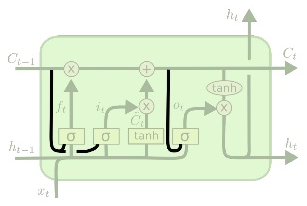
\includegraphics[width=4cm]{images/lstm-peepholes.png}
    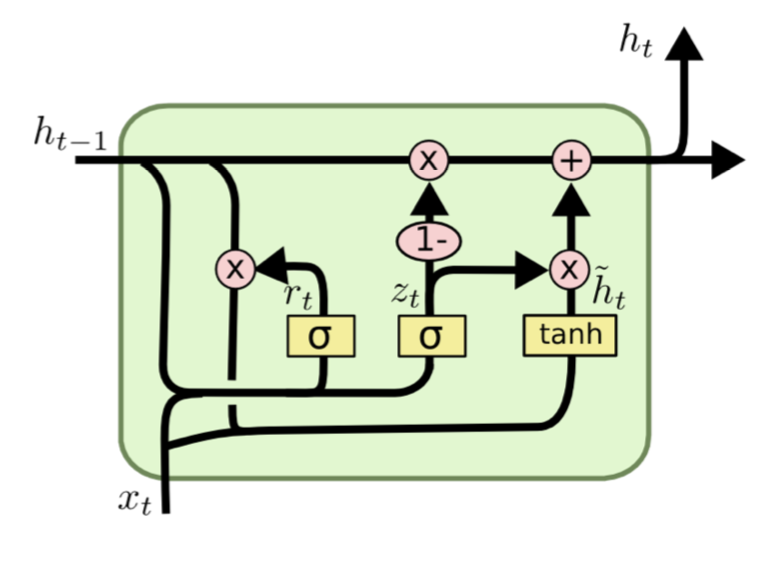
\includegraphics[width=4cm]{images/gru.png}

    
    \tab $i_t=\sigma(W^{(i)}x_t+U^{(i)}h_{t-1})$ input gate\\
\textbf{With peepholes:} $i_t=\sigma(W_i\cdot [C_{t-1},h_{t-1}, x_t]+b_i)$\\
    \tab $o_t=\sigma(W^{(o)}x_t+U^{(o)}h_{t-1})$ output gate \\
\textbf{With peepholes:} $o_t=\sigma(W_o\cdot [C_{t-1},h_{t-1}, x_t]+b_o)$\\
    \tab $f_t=\sigma(W^{(f)}x_t+U^{(f)}h_{t-1})$ forget gate\\
\textbf{With peepholes:} $f_t=\sigma(W_f\cdot [C_{t-1},h_{t-1}, x_t]+b_t)$\\
    \tab $\Tilde{c}_t=\tanh(W^{(c)}x_t+U^{(c)}h_{t-1})$ preparing input to add to memory\\
    \tab $c_t=f_t\odot c_{t-1}+i_t\odot \Tilde{c}_t$ updating memory (combine stored and new)\\
    \tab $h_t=o_t\odot\tanh(c_t)$ output
    
    Where $\odot$ is point-wise multiplication between vectors.
    
    \textbf{Gated memory units:}:

    
    $z_t=\sigma(W_z \cdot [h_{t-1},x_t])$
    $\quad r_t=\sigma(W_r \cdot [h_{t-1},x_t])$\\
    $\Tilde{h}_t=tanh(W \cdot [r_t * h_{t-1},x_t])$
    $\quad h_t=(1-z_t)*h_{t-1}+z_t*\Tilde{h}_t$

    
    \subsubsection{Recursive Networks}
    \label{ssub:recursivenetworks}
    Recurrent = linear chain structure, depth eff. $\vO(n)$, $\vh^t=F(\vh^{t-1},\vx^t)$\\
    Recursive = tree structure, $\vO(\log n)$, $\vh^n=F(\vh^\text{n.left},\vh^\text{n.right})$.\\
    Learn composition $F:\R^d\times\R^d\xrightarrow{}\R^d$, then applied at each inner node of the tree. Application of recursive networks: sentiment analysis.
 % Lecture 09

% Lecture 10
\subsection{Autoencoders}
\label{sub:autoencoders}

    \subsubsection{Autoencoders}
    \label{ssub:autoencoders}
    Given data points $\vx\in\R^n, i=1,...,k$.
    
    \textbf{Goal:} compress data into $m$-dimensional ($m\leq n$) representation.
    
    \textbf{Linear Autoencoder}: $\vx\overset{\vC}{\mapsto}\vz\overset{\vD}{\mapsto}\hat{\vx}\overset{\cR}{\mapsto}\frac{1}{2}\lVert\vx-\hat{\vx}\rVert^2$, choose $\vC,\vD$ s.t. 
    
    \tab$\frac{1}{2k}\sum\limits^k_{i=1}\lVert\vx_i-\vD\vC\vx_i\rVert^2\xleftarrow{}\min$
    
    \textbf{Optimal Linear Compression}: 
    
    \tab Proposition: Given data $\vX=\vU\cdot\diag(\sigma_1,\ldots,\sigma_n)\cdot \vV\T$. The choice $\vC=\vU_m\T$ and $\vD=\vU_m$ minimizes the squared reconstruction error of a two-layer linear auto-encoder with $m$ hidden units.
    \textbf{Proof}: 
    
    \tab $\vD\vC\vX=\underbrace{\vU_m}_\text{1st} \underbrace{\vU_m\T}_\text{2nd}\underbrace{\vU\vSi\vV\T}_\text{data}=\vU_m\lbrack\vI_m\>\>\> \mathbf{0} \rbrack \vSi \vV\T=\vU_m\lbrack \vSi_m\>\>\> \mathbf{0}\rbrack\vV\T$\\
    \tab $\phantom{\vD\vC\vX}=\vU_m\vSi_m\vV_m\T$
    
    Comment: note that we can do weight sharing between the decoder and the encoder networks: $\vD=\vC^\top$
    
    \textbf{Principal Component Analysis}: Assume we have centered the data
    
    \tab $\vx_i\mapsto\vx_i-\frac{1}{k}\sum^k_{i=1}\vx_i$
    
    $\Rightarrow \vS\coloneqq\vX\vX\T\in\R^{n\times n}$ is the sample covariance matrix
    
    $\Rightarrow\vS=\vU\vSi\vV\T\vV\vSi\vU\T=\vU\vSi^2\vU\T$
    
    $\Rightarrow$ columns of $\vU$ are eigenvectors of covariance matrix.
    
    $\Rightarrow\vU_m\vU_m\T$ is projection to $m$ principcal components of $\vS$
    
    \tab This is equivalent to PCA.
    
    \textbf{Regularized Autoencoder}: Can use L2 norm (ability to learn ``overcomplete'' codes), L1 norm (code sparseness), or contractive autoencoders ($\Omega(\vz)=\lambda\lVert \pdv{\vz}{\vx} \rVert^2_F$ penalizes Jacobian and generalizes weight decay)
    
    \textbf{Denoising Autoencoder}: Perturb inputs $\vx\mapsto\vx_\eta$, where $\vet$ is a random noise vector (e.g. additive (white) noise). \textbf{Idea}: learn robust under noise features.
    
    \tab $\vx_\eta=\vx+\vet,\>\>\vet\sim\cN(\mathbf{0},\sigma^2,\vI)$, $\min\xrightarrow{}\E_{\vx}\E_{\vet} \lbrack\ell(\vx,(H\circ G)(\vx_{\vet})) \rbrack$
    
    \tab Hope: $\lVert\vx-\vx_{\vet} \rVert^2 > \lVert\vx - H(G(\vx_{\vet}))\rVert^2 \Rightarrow$ de-noising
    
    
    
    \subsubsection{Factor Analysis}
    \label{ssub:factoranalysis}
    
    \textbf{Latent Variable Models}: Generic way of defining probabilistic i.e. generative models: latent variable models.
    
    \tab 1) Latent variable $\vz$, with distribution $p(\vz)$
    
    \tab 2) Conditional models for observables $\vx$, $p(\vx|\vz)$
    
    \tab 3) Observed data model: integrating/summing out latent variables:
    
    \tab $p(\vx)=\int p(\vz)p(\vx|\vz)\mu(d\vz) = \begin{cases} \mu = \text{ Lebesgue, } & \int p(\vz)p(\vx|\vz)d\vz \\ \mu=\text{ counting, } & \sum_\vz p(\vz)p(\vx|\vz) \end{cases}$
    
    Simple discrete model: mixture model
    
    \tab $\vz\in \{1,\ldots,K\},\> p(\vz)=$ mixing proportions.
    
    \tab $p(\vx|\vz)$: conditional densities (e.g. Gaussians)
    
    \textbf{Linear Factor Analysis}: 
    \tab Latent variable \emph{prior} $\vz\in\R^m$, $\vz\sim\cN(\mathbf{0},\vI)$\\
    Linear \emph{observation model}, $\vx\in\R^n$ \\
    \tab$\vx=\vmu+\vW\vz+\vet,\>\vet\sim\cN(\mathbf{0},\vSi),\>\vSi\coloneqq\diag(\sigma^2_1,\ldots,\sigma^2_n)$
    
    \tab $\vet$ and $\vz$ are independent, typically: $m<n$ (fewer factors than features), few factors account for dependencies between many observables, MLE for $\mu$ on training set: $\hat{\vmu}=\frac{1}{k}\sum^k_{i=1}\vx_i$ (can assume data is centered)
    
    \textbf{Proposition:} in the factor analysis model $\vx \sim \cN(\vmu, \vW\vW^\top+\bf{\Sigma})$
    
    \textbf{Moment Generating Functions}: of random vector $\vx$:
    
    \tab $M_x:\R^n\xrightarrow{}\R,\> M_\vx(\vt)\coloneqq\E_{\vx}\exp \lbrack \vt\T \vx \rbrack \>\>\>\>(= \int^\infty_{-\infty}\vt\T \bar{\vx} \cdot f(\bar{\vx}) \> d\bar{\vx})$
    
    \emph{Uniqueness theorem}: If $M_\vx,\>M_\vy$ exist for RVs $\vx,\vy$ and $M_\vx=M_\vy$ then (essentially) $p(\vx)=p(\vy)$.
    
    $M_\vx$ represents \emph{moments} of $\vx$ in the following way: $k_1,\ldots,k_n\in\mathbb{N}$,
    
    \tab $\E \lbrack x^{k_1} \cdots x^{k_n} \rbrack=\frac{\partial^k}{\partial t^{k_1}_1\cdots \partial t^{k_n}_n}M_\vx \bigr|_{\vt=0}$
    
    Moment generating functions can be used to deal with \emph{sums of i.i.d. random variables}: $M_{\vx+\vy}=M_\vx \cdot M_\vy$
    
    \textbf{Multivariate Gaussian:} $\bf{\Sigma}$ is variance-covariance matrix: $\vE(\vx-\vmu)(\vx-\vmu)^\top$
    
    \tab $\text{PDF}=p(\vx;\vmu,\bf{\Sigma})=\frac{\exp\big[-\frac{1}{2}(\vx-\vmu)^\top\bf{\Sigma}^{-1}(\vx-\vmu)\big]}{\sqrt{(2\pi)^n \cdot \text{det}(\bf{\Sigma})}}$
    
    Moment generating function:
    $M_{\vx}(\vt)=\exp\Big[\vt^\top\vmu+\frac{1}{2}\vt^\top\bf{\Sigma}\vt\Big]$
    
    % \textbf{Maximum Likelihood Estimation}
    
    \subsubsection{Deep Gaussian Models}
    \label{ssub:deepgaussianmodels}
    
    Generalize factor analysis with \emph{depth}. 
    
    Noise variables: $\vz^l \overset{\text{iid}}{\sim} \cN(\mathbf{0},\vI),\>l=1,\ldots,L$
    
    Hidden activities (top-down $\vh^L\xrightarrow{}\vh^1$:
    
    \tab $\vh^L=\vW^L\vz^L,\>\> \vh^l=\underbrace{F^l(\vh^{l+1})}_\text{deterministic}+\underbrace{\vW^l\vz^l}_\text{stochastic}$
    
    Hidden layer (conditional) distribution [vs factor analysis] \\
    \tab $\vh|\vh^+\sim\cN\bigr(F(\vh^+),\vW\vW\T  \bigr)\>\>\lbrack\text{ vs. } \vx|\vz\sim\cN(\vmu,\vW\vW\T+\vSi)  \rbrack$
    
    \textbf{Generative Model Estimation}: We assume that, for a given $\vx$, $q(\vz|\vx)$ is fixed (part of ELBO). How can we optimize $\theta$?
    
    Sample noise variables $(\vz^1,\ldots,\vz^L)\sim q(\vz|\vx)$. Perform backpropagation and SGD step for $\theta$.
    If $q$ is simple, sampling is efficient (no MCMC needed). Unbiased estimation of gradient, small variance overhead. Maybe even be beneficial (training with noise).
    
    \textbf{Stochastic Backpropagation}: Optimizing over $q$ involves gradients of expectations. How does a change of the $q$-distributions change $q$-averages?
    
    \tab $\vz\sim \cN(\vmu,\vSi),\> f:$ smooth and integrable, then\\
    \tab $\nabla_{\vmu} \E \lbrack f(\vz) \rbrack = \E \lbrack \nabla_\vz f(\vz) \rbrack$, $\nabla_{\vSi} \E \lbrack f(\vz) \rbrack=\frac{1}{2} \E \lbrack \nabla^2_{\vz} f(\vz) \rbrack$
    
    via integration by parts:
    
    \tab $\nabla_{\vmu} \E f(\vz) = - \int \nabla_{\vz} \cN (\vmu,\vSi)f(\vz)d\vz=\int\cN(\vmu,\vSi)\nabla_{\vz}f(\vz)d\vz$
    
    \tab (used: $\int f(\vz)\nabla_{\vmu}p(\vz)d\vz   \overset{\text{Gaussian}}{=}-\int f(\vz) \nabla_{\vz}p(\vz)d\vz) $\\
    \tab $\phantom{\text{(used: } f(\vz)\nabla_{\vmu}p(\vz)d\vz}= \int \nabla_{\vz}f(\vz) p(\vz)d\vz) - \underbrace{\lbrack f\cdot p \rbrack^\infty_{-\infty}}_{=0\text{ ``sloppy''}} = \E \lbrack \nabla_{\vz} f(\vz)\rbrack$
    
    \textbf{Deep Latent Gaussian Models}: 2 coupled networks: top-down (generative) and bottom-up (recognition). Forward pass: deterministic recognition, sampled generative. Backward pass: deterministic, but: stochastic backprop.
 % Lecture 10
% Lecture 11
\subsection{Density Estimation \& GAMs}
\label{sub:densityestimationandgams}

\subsubsection{Density Estimation}
\label{ssub:densityestimation}

Standard problem in statistics and unsupervised learning: learn the distribution of the data. Classically: parametric familiy of densities $p(\theta),\>\>\theta\in\Theta$.

MLE: $\theta^* \overset{\text{max}}{\xrightarrow{}} \E \lbrack \ln p_\theta (\vx) \rbrack,\>\> \vx\sim p(\vx)$. In practice: expectation w.r.t. empirical distribution

\textbf{Prescribed models}: Ensure that $p_\theta$ defines a proper density $\int p_\theta(\vx)d\vx=1$

Trivial for models like exponential families. Impractical for complex models (Markov nets, DNNs). What are strategies for more complex models?

\textbf{Latent Variable Models}:

Classicaly: Define complex models via marginalization of a latent variable model

\tab $p_\theta(\vx)=\int p_\theta(\vx,\vz)d\vz$

EM algorithm (ELBO: evidence lower bound)

\tab $\log p_\theta(\vx)\geq \E_{q} \lbrack \log p_\theta (\vx,\vz) \rbrack +D_{\text{KL}}(q(\vz)||p_\theta(\vz)) \overset{\max\E}{\xleftarrow{}}\theta,q$

\tab optimal $q(\vx;\vz)=p_\theta(\vz|\vx)$ (posterior) not always tractable

\emph{Variational inference}: further approximation. Restrict to simpler families of distribution (weakening of ELBO), amortized inference $\Rightarrow$ variational auto-encoders.

\textbf{Unnormalized models}: Represent improper density functions:\\ \tab$\underbrace{\bar{p}_\theta(\vx)}_\text{represented}=\underbrace{c_\theta}_\text{unknown}\cdot \underbrace{p_\theta(\vx)}_\text{normalized}$

Can't use log-likelihood as scaling of $\bar{p}_\theta$ will cause unbounded likelihood. Alternative estimation method for unnormalized models?

\textbf{Score matching}: Is there an operator we can apply to $\bar{p}_\theta$ which does not depend on normalization? Score matching

\tab $\psi_\theta\coloneqq\nabla\log \bar{p}_\theta,\> \psi=\nabla \log p$

Minimize criterion: $J(\theta)=\E \lVert \psi_\theta - \psi \rVert^2$

Equivalently (eliminate $\psi$ using integration by parts):\\
\tab$J(\theta) \overset{\pm c}{=} \E \lbrack \sum_i \partial_i \psi_{\theta,i}-\frac{1}{2}\psi^2_{\theta,i}\rbrack$

Expectation approximated by sampling.

\textbf{Implicit Models}: Statistical models via: \emph{generating stochastic mechanism} or \emph{simulation process}.

\tab Latent code $\R^d\ni\vz\sim\pi(\vz),$ e.g. $\pit(\vz)=\cN(\mathbf{0},\vI)$\\
\tab parameterized mechanism $F_\theta: \R^d\xrightarrow{}\R^m$\\
\tab induced distribution $\R^m \ni \vx\sim p_\theta(\vx)$\\
\tab sampling is easy: random vector + forward propagation

\textbf{Noise Contrastive Estimation}: \emph{bootstrap} generative models via classification problems. Reduce density estimation to binary classification. Define probability ($p_n$: ``contrastive'' distribution: known distribution of negative samples, say ``everything but dogs'' and $p(\vx)$ is ``dogs'')

\tab $\Tilde{p} (\vx,y=1)=\frac{1}{2}p(\vx),\> \Tilde{p}(\vx,y=0)\frac{1}{2}p_n(\vx)$

Probabilistic classifier (induced by $\bar{p}_\theta$)

\tab $q_\theta = \frac{\alpha \bar{p}_theta}{\alpha \bar{p}_\theta + p_n},\> \alpha>0$.

Bayes optimal if $\alpha\bar{p}_\theta=p$. Minimize logistic loss with regard to $\theta$ and $\alpha>0$

This estimator is consistent! It is \emph{sometimes} statistically efficient, but generally \underline{no}.

\subsubsection{Generative Adversarial Models}
\label{ssub:gams}

Classification problem: distinguish between data \& model.

\tab $\Tilde{p}_\theta (\vx,y=1)=\frac{1}{2}p(\vx),\> \Tilde{p}_\theta(\vx,y=0)\frac{1}{2}p_n(\vx)$

Bayes optimal classifier: posterior $q_\theta=p/(p+p_\theta)$.

Train generator via minimizing the logistic likelihood:

\tab $\theta \overset{\min}{\xrightarrow{}}\ell^*(\theta)\coloneqq\E_{\Tilde{p}_\theta} \lbrack y \ln q_\theta(\vx) + (1-y)\ln(1-q_\theta(\vx))\rbrack$

Minimize Jensen-Shannon Divergence to get $\ell^*=\text{JS}(p,p_\theta)-\ln 2$

Generator's goal: generate samples that are \emph{indistinguishable from real data}, even for the best possible classifier. In general this in inaccessible, so we define a classficiation model:

\tab $q_\phi:\vx\mapsto\lbrack 0;1 \rbrack,\> \phi\in\Phi$.

Define objective via bound: \\
\tab$\ell^*(\theta)\geq \sup_{\phi\in\Phi}\ell(\theta,\phi),\> \ell(\theta,\phi)\coloneqq\E_{\Tilde{p}_\theta} \lbrack y\ln q_\phi(\vx) + (1-y)\ln(1-q_\phi)\vx))\rbrack$

Find best classifier within restricted family. Typically: $\Phi=$ weight space of DNN. Training objective is defined implicitly over $\sup$.

\textbf{Optimizing GANs}: Saddle point problem

\tab $\theta^*\coloneqq \argmin_{\theta\in\Theta} \{\sup_{\phi\in\Phi} \ell(\theta,\phi)\}$. Explicitly performing inner $\sup$ is impractical. 

SGD as a heuristic (may diverge!):

\tab $\theta^{t+1}=\theta^t-\eta\nabla_\theta\ell(\theta^t,\phi^t)$

\tab $\phi^{t+1}=\phi+\eta\nabla_\phi\ell(\theta^{t+1},\phi^t)$

\textbf{Evaluating GANs}: Conceptual question: how to measure \emph{quality} of implicit models? likelihood-based method not valid for implicit models. Trade-offs: noisy samples(e.g. blurry images), but adequate representation of variability. Faithful (as in: good looking) samples, but lack of representation (``mode dropping''). Which is better?


% 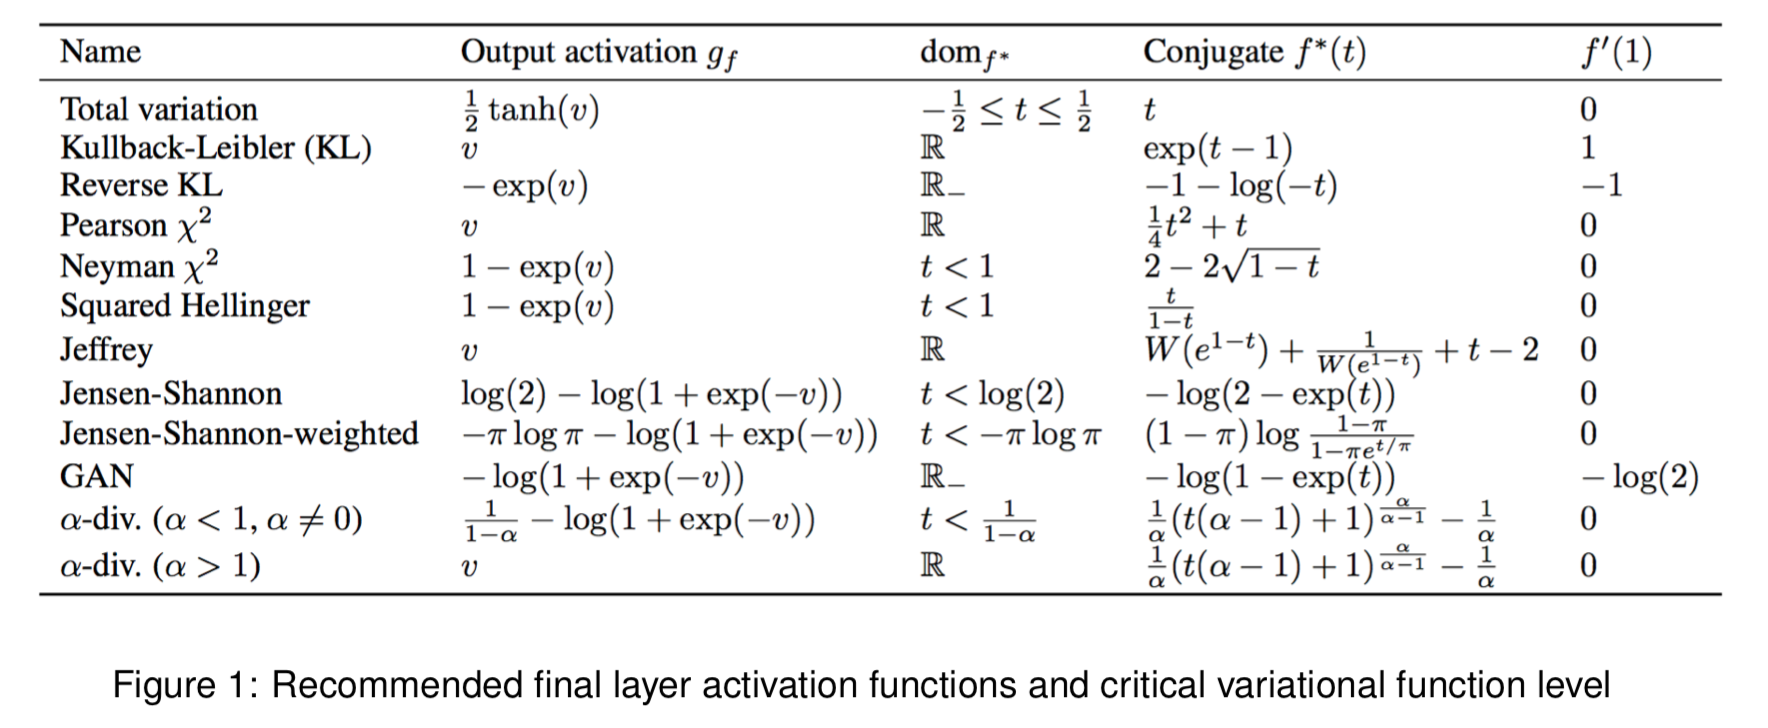
\includegraphics[scale=.25]{images/f-divergences.png} % Lecture 11
\section*{Tricks of the trade}
\subsection*{Matrix Things}
\textbf{SVD:} Suppose $\vM$ is a $m \cross n$ matrix whose entries come from the field $K$, which is either the field of real numbers or the field of complex numbers. There exists a factorization, called a 'singular value decomposition' of $\vM$, of the form
$ \mathbf {M} =\mathbf {U} {\boldsymbol {\Sigma }}\mathbf {V} ^{*}$
where $\vU$ is an $m \cross m$ unitary matrix over $K$ (if $K = \mathbb {R}$ , unitary matrices are orthogonal matrices), $\boldsymbol {\Sigma }$ is a diagonal $m \cross n$ matrix with non-negative real numbers on the diagonal, $\vV$ is an $n \cross n$ unitary matrix over $K$, and $\vV^{∗}$ is the conjugate transpose of $\vV$.
The diagonal entries σi of $\boldsymbol {\Sigma }$ are known as the singular values of $\vM$. A common convention is to list the singular values in descending order.\\
\textbf{Diagonalization}\\
\textbf{Matrix calculus}\\
\tab$(\vA+\vB)'=\vA'+\vB'$, \tab$(\vA\vB\vC)'=\vA'\vB\vC+\vA\vB'\vC+\vA\vB\vC'$,\\
\tab$(\vA^n)'=\vA'\vA^{n-1}+\vA\vA'\vA^{n-2}+\ldots+\vA^{n-1}\vA'$,\\
\tab$(\vA\inv)'=-\vA\inv\vA'\vA\inv$, $(\det(\vA))'=\Tr(\vA'\vA)$,\\
\tab$(\vA\vx)'=\vA\T$, $(\vx\T\vA)'=\vA$, $(\vx\T\vx)'=2\vx$, \tab$(\vx\T\vA\vx)'=\vA\vx+\vA\T\vx$


\textbf{Matrix math}\\
\tab$(\vA\vB)\T=\vB\T\vA\T$

\textbf{Trace identities and differention rules:}\\
$\vv^\top\vw = \sum\limits_i v_iw_i=\Tr(\vA+\vB) \quad \Tr(\vA+\vB)=\Tr(\vA)+\Tr(\vB)$\\
$\vE\Tr(\vX)=\Tr\vE[\vX]$\\
$ \nabla_\vA\Tr(\vA\vA^\top)=2\vA, \quad \nabla_\vA\Tr(\vA\vB)=\vB^\top$

\textbf{Positive definite}:

\tab$\vA$ is positive definite if $\vx\T\vA\vx > 0,\>\> \forall \vx\neq0$

\tab$\vA$ is indefinite if it contains positive and negative eigenvalues.

\textbf{Finding Eigenvalues}:

\tab $\det(\vA - \lambda \vI)=0$ and find values of $\lambda$ that make this true. To get eigenvector for $\lambda_i$, plug $\lambda_i$ into $\vA - \lambda_i \vI = \vB$ and solve $\vB\bar{\vX}=\mathbf{0}$. (Do row reduction to get one equation containing eigenvector components $x_i$, find values for each $x_i$ to make the equation true. Stack these $x_i$ to get the eigenvector for $\lambda_i$. 

\tab $\det(\vA - \lambda \vI)$

\subsection*{General Math}
\textbf{Derivative rules}\\
$\tan(x)\xrightarrow{}\sec^2(x),\>a^x\xrightarrow{}\ln(a)a^x,\>f/g\xrightarrow{}(f'g-g'f)/g^2$



\textbf{Sigmoid Derivative}: $\dv{\sigma(x)}{x} = \sigma(x)(1-\sigma(x))$\\

\textbf{Integration by parts}: $\int u\>dv=uv - \int v\>du$

\textbf{Fundamental Theorem of Calculus}: $f(y)-f(x)=\int^y_x\nabla f(\tau) d\tau$

\textbf{Mean}: $\mathbb{E}\lbrack f(x) \rbrack = \int_x x\>f(x)\>dx$ \textbf{Variance:} $\mathbb{E}\lbrack f(x) \rbrack = \mathbb{E} \lbrack f(x)^2\rbrack - \mathbb{E} \lbrack f(x) \rbrack^2$

\textbf{Convexity of $f$ implies}: $f(y)\geq f(x)+\nabla f(x)\T (y-x), \forall (x,y) \in \R^{d\times d}$

\textbf{Cauchy-Schwarz}: $\lvert \langle \vu ,\vv \rangle\rvert^2\leq\langle \vu,\vu\rangle\cdot\langle\vv,\vv\rangle \xrightarrow{} \lvert\langle\vu,\vv\rangle\rvert\leq\lVert\vu,\vv\rVert $.

\textbf{Taylor Expansion}\\
\tab$f(x)=\sum\limits^\infty_{n=0}\frac{f^{(n)}(x_0)}{n!}(x-x_0)^n$ with expansion around $x_0$.

\tab$f(\vw)\approx f(\bar{\vw})+(\vw-\bar{\vw})\T\nabla f(\bar{\vw})+\frac{1}{2}(\vw-\bar{\vw})\T H (\vw-\bar{\vw})$

\textbf{Taylor-Lagrange}:
$f(x)=\sum\limits^n_{k=0}\frac{f^{(k)}(x_0)}{k!}(x-x_0)^k+\int\limits^x_{x_0}\frac{f^{(n+1)}(t)}{n!}(x-t)^n dt$.

\textbf{KL divergence}: $D_\text{KL}(P||Q)=-\sum_i P(i) \log \frac{Q(i)}{P(i)}$

\textbf{Eigenvalues and vectors}: $H\vu_i=\lambda_i\vu_i$\\
Eigenvectors are orthonormal (for real, symmetric): $\vu_i\T\vu_j=\delta_{ij}$

\textbf{Log Likelihood:} $\log\Pi^N_n p(t_n|x_n)=\log\Pi^N_n p(t_n=1|x_n)^{t_n} p(t_n=0|x_n)^{1-t_n}=\sum^N_n t_n \log p(t_n|x_n) + (1-t_n) \log (1-p(t_n|x_n))$

\tab put minus in front to get cross-entropy loss.

\textbf{Probability Names}: $P(Y|X)\xrightarrow{}$ likelihood, $P(X|Y)\xrightarrow{}$ posterior, $P(X)\xrightarrow{}$ prior, $P(Y)\xrightarrow{}$ evidence. Posterior = (likelihood * prior)/evidence

\textbf{Set Theory}\\
Compact: closed and bounded\\
$f\in\cC^{n+1}(\lbrack a,b\rbrack,\R)$: diff. $n+1$ times and is a mapping from $\lbrack a,b\rbrack$ to $\R$

\textbf{Newton's Method}: $\theta(t+1)=\theta(t)-\!\!\!\!\!\underbrace{(\nabla^2\cR)\inv}_\text{inverse Hessian}\!\!\!\!\!\nabla\cR\bigr|_{\theta=\theta(t)}$

\subsection*{Misc. Deep Learning}
\subsubsection*{Loss Functions}
\textbf{L1-norm loss}: least absolute deviations (LAD), least absolute errors (LAE) 

\tab $L=\sum^n_{i=1} \lvert y_i - f(x_i) \rvert$

\textbf{L2-norm loss}: least-squared errors (LSE)

\tab $L=\sum^n_{i=1} \lVert y_i - f(x_i) \rVert^2$

\textbf{L2-regularized}:

\tab $L(x;\theta)=\sum^n_{i=1} \lVert y_i - f(x_i;\theta) \rVert^2 + \lambda\sum_{ij}\theta_{ji}^2$

\textbf{Mean Squared Error}: MSE

\tab $L=\sum^n_{i=1} \lVert y_i - f(x_i) \rVert^2 / n$

\textbf{Cross-Entropy Loss}: log loss

$L=-\log\Pi^N_n p(t_n|x_n)=-\log\Pi^N_n p(t_n=1|x_n)^{t_n} p(t_n=0|x_n)^{1-t_n}=-\bigr(\sum^N_n t_n \log p(t_n|x_n) + (1-t_n) \log (1-p(t_n|x_n))\bigr)$



\section*{Examples}
\subsection*{Ex4 P2: Approximate Hessian for feed-forward NN}
\textbf{Setup}: $a_j=\sum\limits_i w_{ji}z_i$, where $z_i$ is the activation of a unit that sends a connection to unit $j$, and $w_{ji}$ is the weight associated with that connection. Let $h$ be a nonlinear activation function, then $z_i=h(a_i)$. Evaluate second derivatives of the loss, $\frac{\partial^2 L}{\partial w_{ji} \partial w_{lk}}$. Recall the loss function decomposes over samples from the dataset as $L(\cdot)=\sum_n L_n(\cdot)$

\textbf{Compute $\frac{\partial L_n}{\partial w^2_{ij}}$ as a function of $z^2_i$.}\\

\tab$\frac{\partial L_n}{\partial w^2_{ij}}=\frac{\partial}{\partial w_{ji}}\cdot \frac{\partial L_n}{\partial w_{ji}}=\frac{\partial}{\partial w_{ji}}(\frac{\partial L_n}{\partial a_j}\cdot\frac{\partial a_j}{\partial w_{ji}})=\frac{\partial}{\partial w_{ji}}(\frac{\partial L_n}{\partial a_j}\cdot z_i)$\\

\tab Used: $\pdv{a_j}{w_{ji}}=\pdv{\sum_i w_{ji}z_i}{w_{ji}}=z_i$ for one specific $i$. Apply product rule:

\tab$\pdv{}{w_{ji}} (\pdv{L_n}{a_j}\cdot z_i)=\pdv{}{w_{ji}} (\pdv{L_n}{a_j})\cdot z_i+\pdv{L_n}{a_j}\pdv{z_i}{w_{ji}}$. (and $\pdv{z_i}{w_{ji}}=0$ since output of $i$ doesn't depend on $w_{ji}$).

\tab $\pdv{}{w_{ji}} ( \pdv{L_n}{a_j} )\cdot z_i=\pdv{}{w_{ji}} (\pdv{L_n}{w_{ji}})\cdot z_i=\pdv{}{a_j} (\pdv{L_n}{a_j}\pdv{a_j}{w_{ji}})\cdot z_i=\pdv[2]{L_n}{a_j}\cdot z_i^2$

\textbf{Show that:} $\frac{\partial^2 L_n}{\partial a_j^2}=h'(a_j)^2\sum\limits_k\sum\limits_{k'} w_{kj}w_{k'j}\frac{\partial^2 L_n}{\partial a_k \partial a_{k'}}+h''(a_j)\sum\limits_k w_{kj}\frac{\partial L_n}{\partial a_k}$

\tab use (by chain rule): $\pdv{L_n}{a_j} = \sum_k \pdv{L_n}{a_k} \cdot \pdv{a_k}{a_j}$\\
\tab For one specific $k$: $\pdv{a_k}{a_j} = \pdv{\sum_i w_{ki} z_i}{a_j} = \pdv{w_{kj} z_j}{a_j} = h'(a_j) w_{kj}$\\

\tab$\pdv[2]{L_n}{a_z} = \pdv{}{a_j} ( \pdv{L_n}{a_j} ) = \pdv{}{a_j} \bigr( h'(a_j) \sum_k w_{kj} \pdv{L_n}{a_k} \bigr) $\\
\tab$\phantom{\pdv[2]{L_n}{a_z} } = h''(a_j) \sum_k w_{kj} \pdv{L_n}{a_k}+h'(a_j) \sum_k w_{kj} \frac{\partial^2 L_n}{\partial a_k \partial a_j}$\\

Then: $\frac{\partial^2 L_n}{\partial a_k \partial a_j}= \pdv{}{a_k} \cdot \pdv{L_n}{a_j} = \pdv{}{a_k} \bigr(h'(a_j) \sum_{k'} w_{k'j} \pdv{L_n}{a_{k'}} \bigr)$\\

$\phantom{\text{Then: }\frac{\partial^2 L_n}{\partial a_k \partial a_j}}=h'(a_j)\sum_{k'} w_{k'j} \frac{\partial^2 L_n}{\partial a_k' \partial a_k}$

\textbf{Question:} \emph{Assume we can neglect off-diagonal elements in the second-derivative terms. What expression do we get? What's the computational complexity compared to computing the exact Hessian matrix?}

\tab$\pdv[2]{L_n}{a_j} = h'(a_j)^2 \sum_k w^2_{kj} \pdv[2]{L_n}{a_k} + h''(a_j) \sum_k w_{kj} \pdv{L_n}{a_k}$.\\

\tab The computational complexity for this approx. Hessian is $O(W)$ where $W$ is the total number of weights in the network, $O(W^2)$ for the full Hessian.

\begin{figure}[H]
        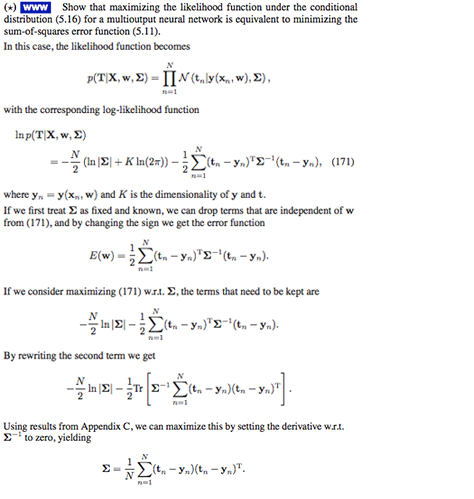
\includegraphics[width=\columnwidth]{images/bishop5-3.png}
        
        \label{fig:my_labeflf}
    \end{figure}

\begin{figure}[H]
        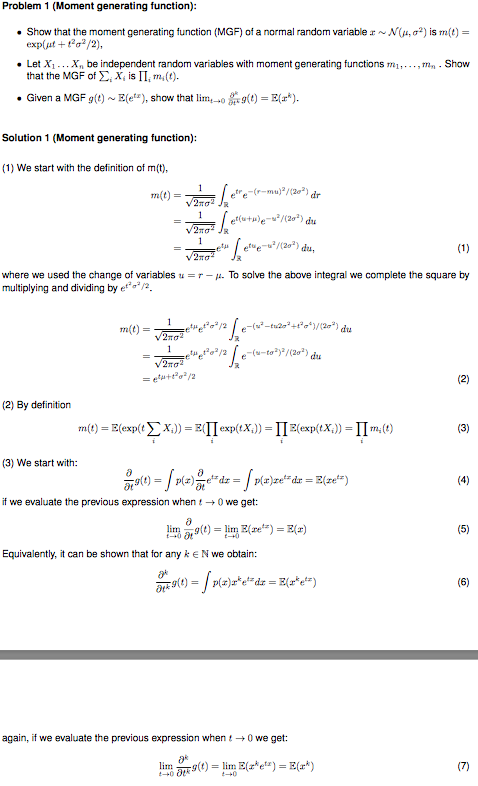
\includegraphics[width=\columnwidth]{images/ex11p1.png}
        
        \label{fig:my_labelf}
    \end{figure}

\subsection{Sanity checks:}
The gradient with respect to a variable should always have the same shape as that variable.

% \textbf{Neat resources: http://cs231n.stanford.edu/slides/2017/}

\section{Sylvester's criterion}
\href{https://en.wikipedia.org/wiki/Sylvester\%27s_criterion}{Aqui!}

A differentiable function of one variable is convex on an interval if and only if the function lies above all of its tangents:
$f(y)\geq f(x)+\nabla f(x)^T(y-x)$

\textbf{Weierstrass theorem:} If f is a given  continuous  function for $a\leq x \leq b$ and if $\epsilon$ is an arbitrary positive quantity, it is possible to construct an approximating polynomial $P(x)$ such that: $|f(x)-P(x)|\leq \epsilon, \quad a\leq x\leq b$ % Miscellaneous


\end{multicols*}
\end{document}